\documentclass[journal]{vgtc}                % final (journal style)
%\documentclass[review,journal]{vgtc}         % review (journal style)
%\documentclass[widereview]{vgtc}             % wide-spaced review
%\documentclass[preprint,journal]{vgtc}       % preprint (journal style)
%\documentclass[electronic,journal]{vgtc}     % electronic version, journal

%% Uncomment one of the lines above depending on where your paper is
%% in the conference process. ``review'' and ``widereview'' are for review
%% submission, ``preprint'' is for pre-publication, and the final version
%% doesn't use a specific qualifier. Further, ``electronic'' includes
%% hyperreferences for more convenient online viewing.

%% Please use one of the ``review'' options in combination with the
%% assigned online id (see below) ONLY if your paper uses a double blind
%% review process. Some conferences, like IEEE Vis and InfoVis, have NOT
%% in the past.

%% Please note that the use of figures other than the optional teaser is not permitted on the first page
%% of the journal version.  Figures should begin on the second page and be
%% in CMYK or Grey scale format, otherwise, colour shifting may occur
%% during the printing process.  Papers submitted with figures other than the optional teaser on the
%% first page will be refused.

%% These three lines bring in essential packages: ``mathptmx'' for Type 1
%% typefaces, ``graphicx'' for inclusion of EPS figures. and ``times''
%% for proper handling of the times font family.

\usepackage{enumerate}

\usepackage{mathptmx}
\usepackage{graphicx}
\usepackage{times}

\usepackage{booktabs}
\usepackage{subfigure}

\usepackage{listings}

\usepackage{afterpage}
\usepackage{url}

%\usepackage[T1]{fontenc}
\usepackage{xcolor}
\definecolor{cornellred}{rgb}{0.7, 0.11, 0.11}
\newcommand{\E}{\textcolor{cornellred}{\textbf{TO DO Edwin}}}
\newcommand{\M}{\textcolor{blue}{\textbf{TO DO Martijn}}}
\newcommand{\changedE}[1]{\textcolor{cornellred}{#1}}
\newcommand{\changedM}[1]{\textcolor{blue}{#1}}

%% We encourage the use of mathptmx for consistent usage of times font
%% throughout the proceedings. However, if you encounter conflicts
%% with other math-related packages, you may want to disable it.

%% This turns references into clickable hyperlinks.
\usepackage[bookmarks,backref=true,linkcolor=black]{hyperref} %,colorlinks
\hypersetup{
  pdfauthor = {},
  pdftitle = {},
  pdfsubject = {},
  pdfkeywords = {},
  colorlinks=true,
  linkcolor= black,
  citecolor= black,
  pageanchor=true,
  urlcolor = black,
  plainpages = false,
  linktocpage
}

%% If you are submitting a paper to a conference for review with a double
%% blind reviewing process, please replace the value ``0'' below with your
%% OnlineID. Otherwise, you may safely leave it at ``0''.
\onlineid{234}

%% declare the category of your paper, only shown in review mode
\vgtccategory{Research}

%% allow for this line if you want the electronic option to work properly
\vgtcinsertpkg

%% In preprint mode you may define your own headline.
%\preprinttext{To appear in an IEEE VGTC sponsored conference.}

%% Paper title.

\title{Tree Colors: color schemes for tree structured data}

%% This is how authors are specified in the journal style

%% indicate IEEE Member or Student Member in form indicated below
\author{Martijn Tennekes and Edwin de Jonge}


\authorfooter{
%% insert punctuation at end of each item
\item
Martijn Tennekes, Statistics Netherlands. E-mail: m.tennekes@cbs.nl.
\item
Edwin de Jonge, Statistics Netherlands. E-mail: e.dejonge@cbs.nl.
}

%other entries to be set up for journal
\shortauthortitle{Biv \MakeLowercase{\textit{et al.}}: Tree Colors: color schemes for tree structured data}
%\shortauthortitle{Firstauthor \MakeLowercase{\textit{et al.}}: Paper Title}

%% Abstract section.
\abstract{
We present a method to map tree structures to colors from the Hue-Chroma-Luminance color model, which is known for its well balanced perceptual properties. The Tree Colors method can be tuned with several parameters, whose effect on the resulting color schemes is discussed in detail. We provide a free and open source implementation with sensible parameter defaults. Categorical data are very common in statistical graphics, and often these categories form a classification tree. We evaluate applying Tree Colors to tree structured data with a survey on a large group of users from a national statistical institute. Our user study suggests that tree color schemes are useful, not only for improving node-link diagrams, but also for unveiling tree structure in non-hierarchical visualizations. %Remarkably we find that Tree Colors do not improve detection of parent-child relations in treemaps in comparison to a standard qualitative color scheme.

%Color is an important means to display categorical data in statistical graphics. Categories are often hierarchically structured in a classification tree, but most color palettes do not take this hierarchy into account. We present a method to map tree structures to colors from the Hue-Chroma-Luminance (HCL) color model. The HCL color space is known for its well balanced perceptual properties. Our study suggest that hierarchical qualitative color palettes are very useful, not only for improving standard hierarchical visualizations such as graphs and treemaps, but also for showing tree structures in non-hierarchical visualizations.
} % end of abstract

%% Keywords that describe your work. Will show as 'Index Terms' in journal
%% please capitalize first letter and insert punctuation after last keyword
\keywords{Color schemes, statistical graphics, hierarchical data.}

%% ACM Computing Classification System (CCS). 
%% See <http://www.acm.org/class/1998/> for details.
%% The ``\CCScat'' command takes four arguments.

\CCScatlist{ 
 \CCScat{H.5.2}{ Information Interfaces and Presentation}%
{User Interfaces}{User-centered design}
}


%% Uncomment below to include a teaser figure.
  \teaser{
  \centering
 \mbox{\subfigure{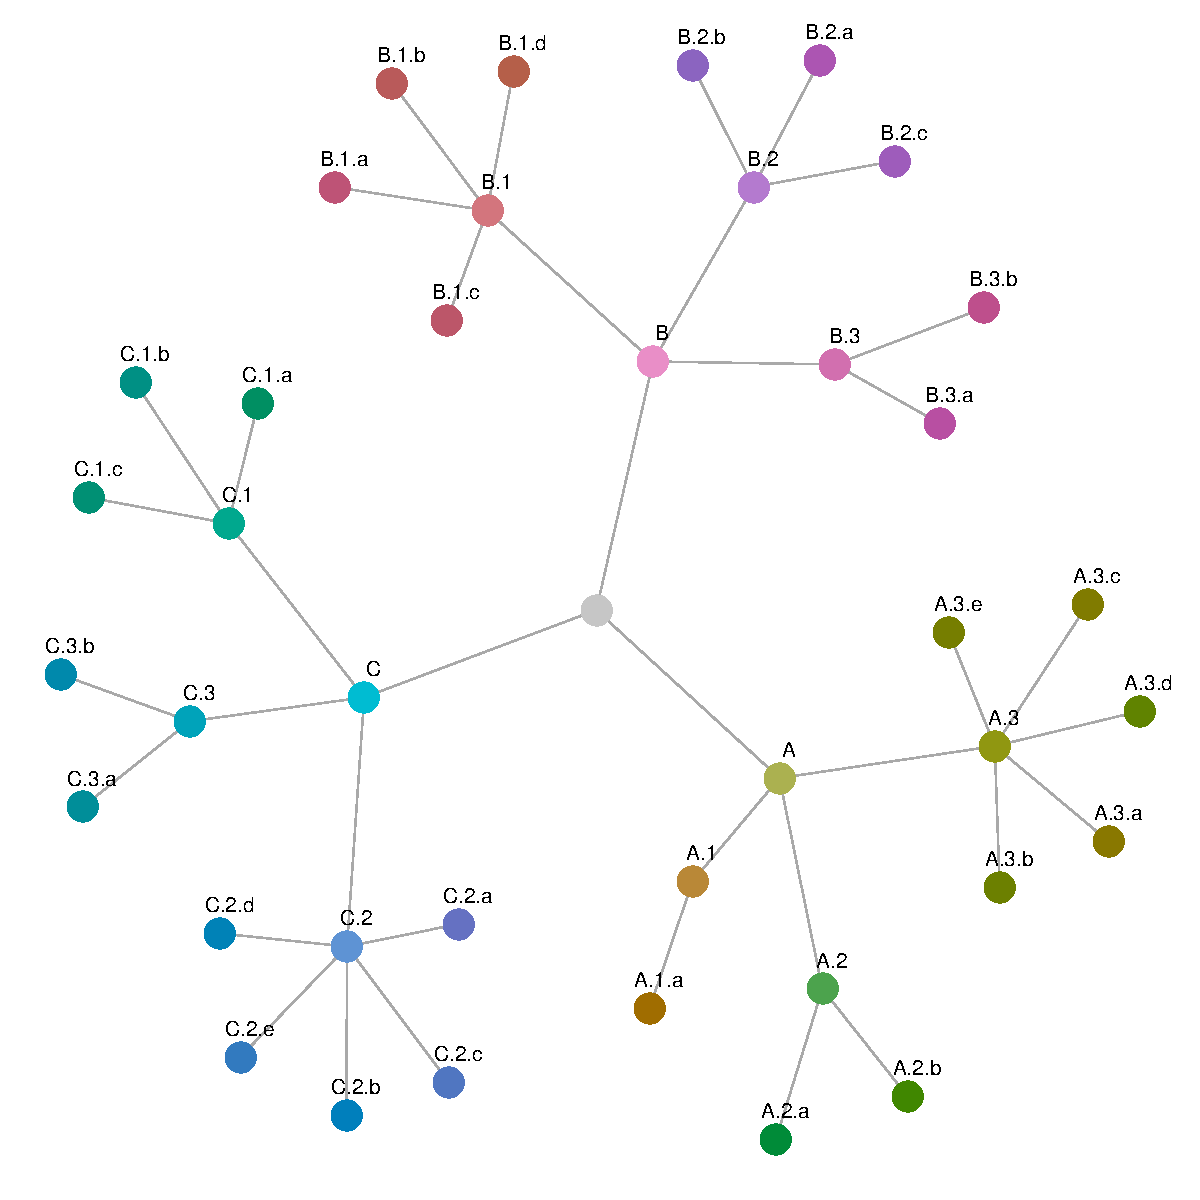
\includegraphics[width=8cm]{Graph_teaser.pdf}}\quad
  \subfigure{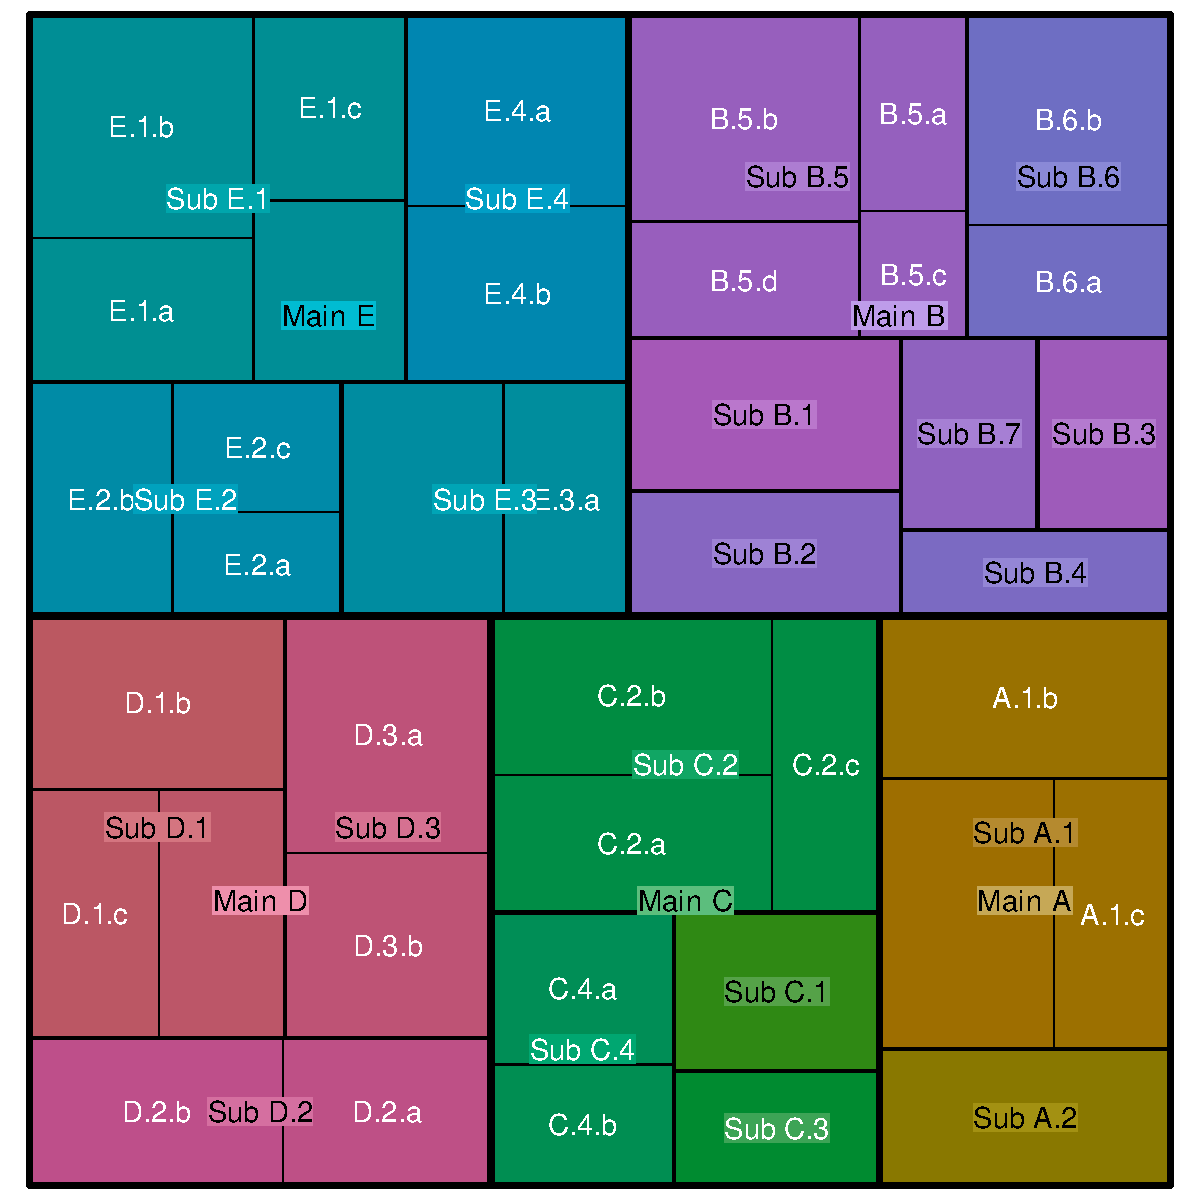
\includegraphics[width=8cm]{Treemap_teaser.pdf}}}
  \caption{Tree Colors applied to a node-link diagram (left) and a treemap (right).}\label{fig:teaser}
  }

%% Uncomment below to disable the manuscript note
%\renewcommand{\manuscriptnotetxt}{}

%% Copyright space is enabled by default as required by guidelines.
%% It is disabled by the 'review' option or via the following command:
% \nocopyrightspace

%%%%%%%%%%%%%%%%%%%%%%%%%%%%%%%%%%%%%%%%%%%%%%%%%%%%%%%%%%%%%%%%
%%%%%%%%%%%%%%%%%%%%%% START OF THE PAPER %%%%%%%%%%%%%%%%%%%%%%
%%%%%%%%%%%%%%%%%%%%%%%%%%%%%%%%%%%%%%%%%%%%%%%%%%%%%%%%%%%%%%%%%


\graphicspath{{../plots/}}


\begin{document}

\lstset{language=R}
%% The ``\maketitle'' command must be the first command after the
%% ``\begin{document}'' command. It prepares and prints the title block.

%% the only exception to this rule is the \firstsection command
\firstsection{Introduction}\label{secintro}

\maketitle
Data are often hierarchically structured. For example business data are typically broken down by economic activity and demographic data by geographic region. Several visual exploration methods of such data use the underlying hierarchical structure, for instance treemaps
\cite{shneiderman1992,tennekes2011b}. Color schemes reflecting the hierarchical structure would be very useful in supporting visual analysis. 
%\changedM{Such palettes could clarify the hierarchical structure of the data. Although this structure is often encoded in the layout, the use of hierarchical colors palettes could make the use of a hierarchical layout less necessary.} \changedE{Such palettes could clarify the chosen layout by emphasizing the tree structure of the data: this makes it possible to relax a tree layout of a node-link diagram, having more space to place the nodes.} 
Such color schemes could clarify the chosen layout by emphasizing the tree structure of the data. For node-link diagrams, this makes it possible to relax its tree layout, having more space to place the nodes and labels.

Assigning colors to categories is far from trivial. On the one hand, qualitative colors should be distinct, but on the other hand they should minimize perceptual bias by preventing the suggestion of non-existent order or proximity. The selection of color schemes for categorical data first depends on the type of data. For nominal data, such as gender or nationality, qualitative color schemes are used, while for ordinal data, such as level of urbanization, sequential or diverging color schemes are used \cite{brewer03, zeileis2009}. However, for hierarchical categories there are no specific guidelines for selecting color schemes, to the best of our knowledge.


%\E In our opinion, a good hierarchical color scheme should have at least have the following properties. First it should assign a unique and distinct (as possible) color to each node of the tree, since each node is a different category. The second property is that the assigned colors should reflect the tree structure: a node should have a similar color to its parent and, by transitivity, its children and siblings.
%Third and last the hierarchical depth of a node should be encoded in its color.

We have designed a hierarchical color scheme with the following properties in mind. First it is a qualitative color scheme that assigns a unique and distinct color to each node of the tree with no perceived order in nodes \cite{brewer03, zeileis2009}. Second, to encode parent-child relations, the color of each node is similar to its parent. Third and last, the depth of a node is reflected in the color of a node. By transitivity the last two properties result in similar colors for siblings.

The color schemes that are generated by our proposed method are called Tree Colors. To ensure well
balanced perceptual properties, we use the Hue-Chroma-Luminance (HCL) space, a transformation of the CIELUV color space, that is designed with the aim to control human color perception~\cite{ihaka2003}. Colors with different hue values are perceptually uniform in colorfulness and brightness, which does not hold for the popular Hue-Saturation-Value (HSV) and HSL color spaces~\cite{zeileis2009}.

We evaluated the Tree Colors method with a user study by comparing it to a color scheme with distinct colors for each main branch of the tree. The results of this study indicate
that Tree Colors can be effective in tree visualizations, especially in tree structured node-link diagrams. However, the results for treemaps
are mixed, and therefore additional research in this area is needed

This paper is outlined as follows. In Section~\ref{secmethod} we describe the proposed method. We provide several applications of statistical graphics that use Tree Colors in Section~\ref{secapplication}. The conducted user study is described in Section~\ref{secuser}. We conclude with a discussion in Section~\ref{secdisc}.

\section{Related work}

Most tree visualizations proposed in literature \cite{schulz2011} use color to a small extent. A visualization technique that uses color as a major attribute is InterRing \cite{yang2002}, a navigation tool with a radial layout. The leaf nodes are assigned different hue values. The color of a parent node is derived by averaging the colors of its children, where larger branches have more weight. An implicit effect of this method is that colors of higher hierarchical levels are less saturated, except for one-child-per-parent branches. 
Hierarchical color schemes are also applied to the Hyperbolic Wheel \cite{lam2012}, an exploration tool for hierarchical data.  These color schemes are abstracted from the Hue-Saturation-Lightness (HSL) space, where brightness decreases proportional from root to leaf nodes, and where child nodes inherit the hue values from their parent nodes and add small hue values to distinct them from their siblings. However, hue values of nodes in the same hierarchical layer may be overlapping.

Several websites contain examples of visualizations that use color to encode tree structure. For example newsmap.jp~\cite{newsmap} aggregates news and presents a treemap of news to its users. 
The color of each news item indicates one of seven news categories. Each news category has a fixed hue value, and the colors of items within a news category differ in chroma and luminance to make the rectangles more distinct and attractive. In contrast, when using Tree Colors, sibling nodes have different hues but equal luminance and chroma values. Moreover, the used color scheme only supports two hierarchical layers, namely the news categories and the items within each category.
IBM's Many Eyes \cite{manyeyes} uses HSV color schemes for treemaps. The colors vary in hue but all have equal saturation and value. Nodes within a group have similar hue values. This is comparable to Tree Colors, although a different color space model is used. Furthermore, like newsmap.jp, the Many Eyes color scheme is restricted to one grouping.

While there seems to be a need for tree color schemes, to the best of our knowledge no guidelines or 
descriptions are given in literature for constructing such color schemes.

\section{Method}\label{secmethod}
Our method maps a tree structure on colors in HCL space, which is a transformation of the CIELUV color space, such that it reflects the hierarchical properties of the tree. We use the hue parameter $H$, with range [0, 360], for the tree structure, where the hue of each child node resembles the hue of its parent. The chroma and luminance parameters $C$ and $L$, both with range [0, 100], are used to discriminate the different hierarchical levels.

An example of Tree Colors applied to a tree drawn with a radial layout is shown in Figure~\ref{fig:graph}. 
Although other layouts may be more suitable to highlight tree structure, for instance the Fruchterman-Reingold algorithm~\cite{Fruchterman91} applied in the node-link diagram in Figure~\ref{fig:teaser}, the applied radial Reingold-Tilford layout~\cite{reingold81} preserves the original order of nodes in each hierarchical layer, which is in this case purely alphabetical. This layout helps to illustrate the assignment of Tree Colors to the nodes of a tree. 
%Radial layouts have proven to be very useful in many tree visualizations methods and navigation tools \cite{schulz2011}.

\begin{figure}[tb]

  \centering
  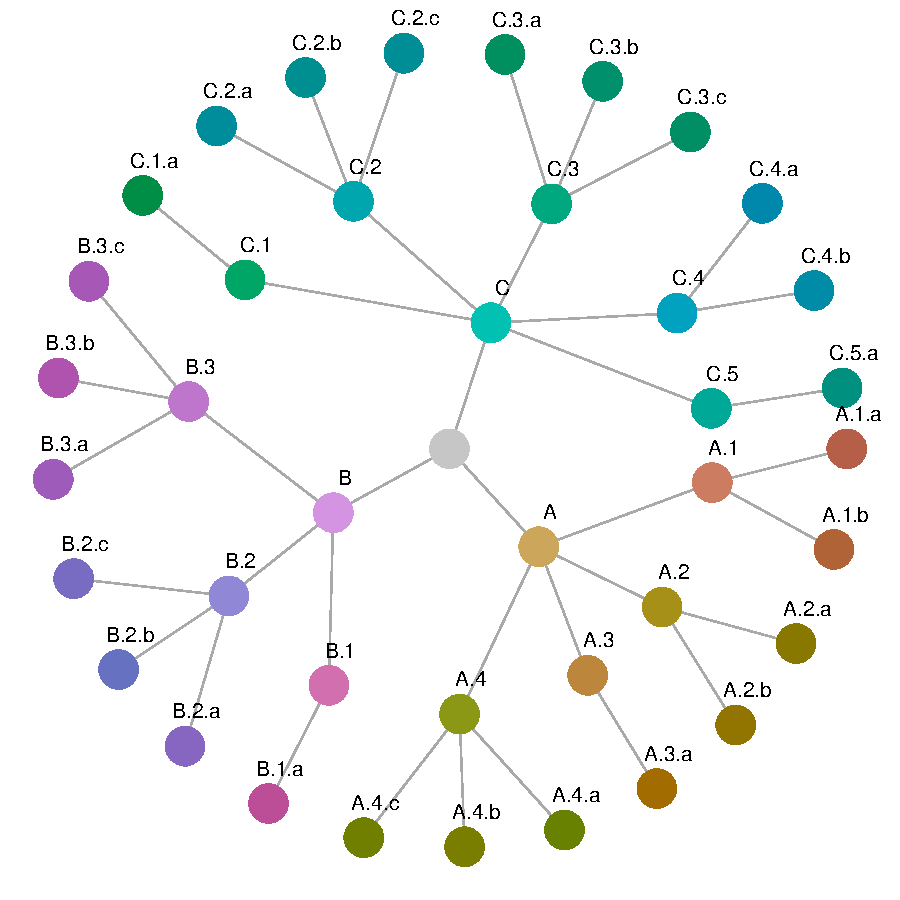
\includegraphics[width=3.2in]{HCPgraph.pdf}
  \caption{Radial layout of a tree colored with Tree Colors.}\label{fig:graph}

\end{figure}

\subsection{Hue values}
Hue values are selected using the following recursive algorithm that assigns to each node 
$v$ of a tree structure a hue value $H_{v}$. 
The inputs for the algorithm are a hue range $r$, a hue fraction $f$, a boolean permutation flag  
\texttt{perm} and a boolean reverse flag \texttt{rev}.
The root of a tree starts with hue range $r=[H_{start}=0, H_{end}=360]$:

\smallskip{\textbf{AssignHue($v$, $r$, $f$,} \texttt{perm}\textbf{,} \texttt{rev}\textbf{)}}%
\begin{enumerate} \itemsep1pt \parskip0pt 
\parsep0pt
\item Select the middle hue value in $r$ as the hue value of node $v$, which is $H_v$ \footnote{The root node itself is colored gray, so its hue is irrelevant.}.
\item Let $N$ be the number of child nodes of $v$. If $N>0$ :
\begin{enumerate}[i] \itemsep1pt \parskip0pt 
\parsep0pt
\item divide $r$ in $N$ equal parts $r_i$ with $i=1,\ldots,N$;
\item if \texttt{perm} then permute the $r_i$'s;
\item if \texttt{rev} then reverse the even-numbered $r_i$'s;
\item reduce each $r_i$ by keeping its middle fraction $f$;
\item for each child node $v_i$ DO AssignHue($v_i$, $r_i$, $f$, \texttt{perm}, \texttt{rev}).
\end{enumerate}
\end{enumerate}

\begin{figure}[tb]
  \centering
  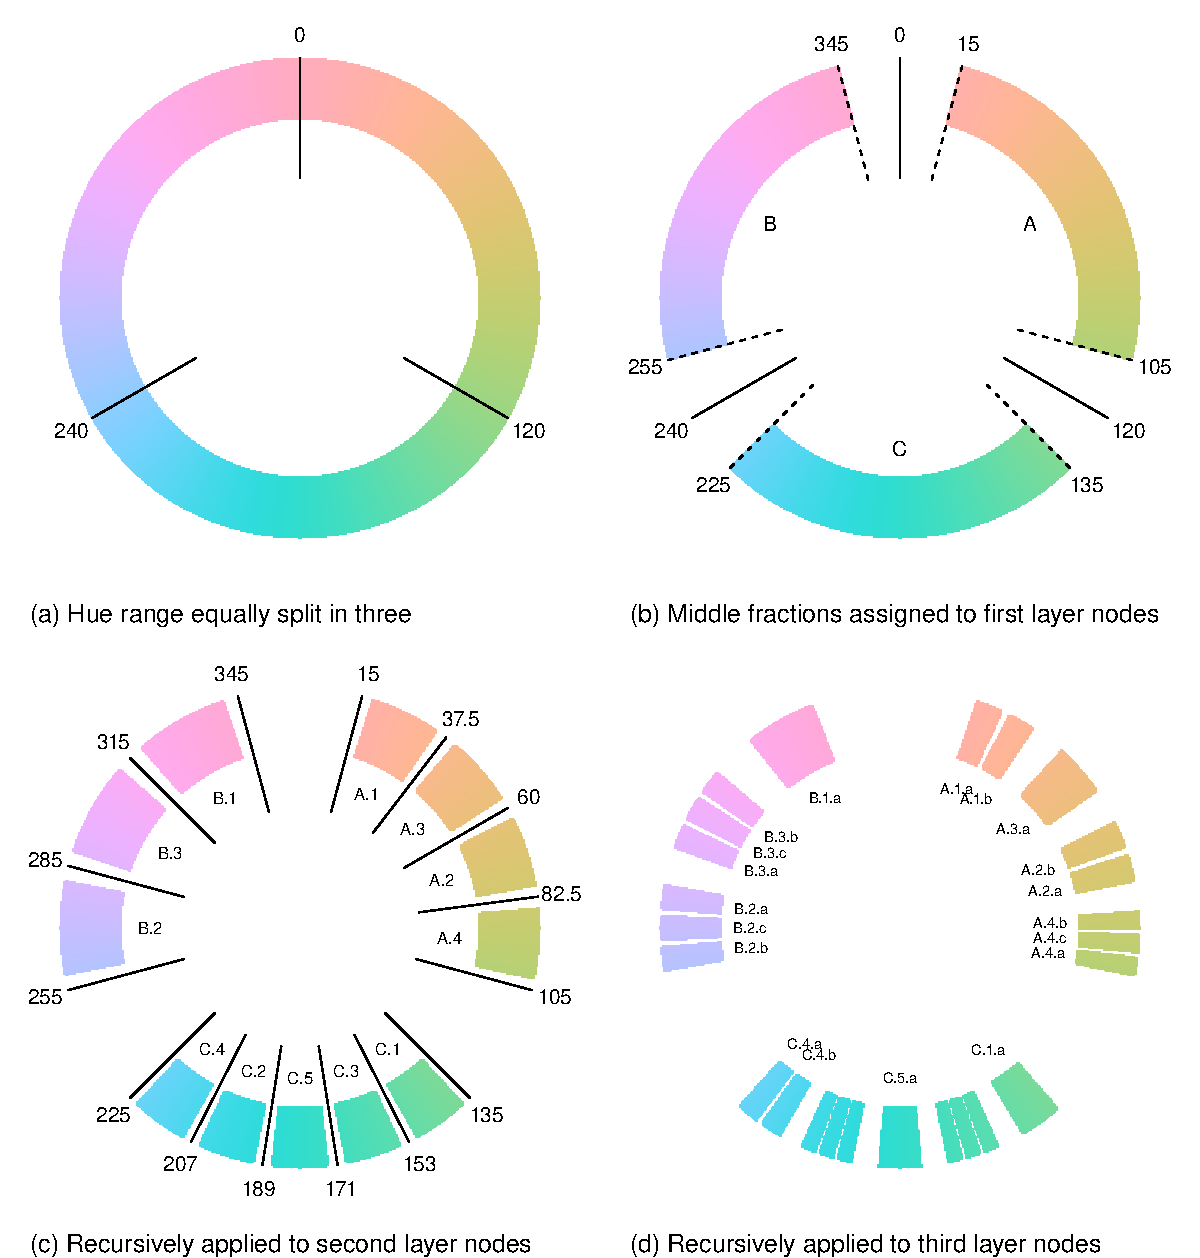
\includegraphics[width=3.5in]{hcl_method2.pdf}
  \caption{Assignment of hue values.}\label{fig:wheel}
\end{figure}

This algorithm is illustrated in Figure~\ref{fig:wheel}. In (a) the full hue range (for a constant $C=60$ and $L=70$)  is split in three equal parts, since the root node has three children. Of each part, only the middle fractions ($f$, with a default value of 0.75) are kept in (b) and assigned to A, B, and C. For example, from the part between 0 to 120 degrees, only the $120*0.75=90$ degrees in the middle, so from 15 to 105 degrees, are kept and assigned to A. In (c) and (d) these steps are recursively taken for the deepest two hierarchical layers.

\subsubsection{Hue permutations and reversals}\label{sechueperm}

In most hierarchical structures, there is no order between siblings. 
When the nodes in such structure are plotted in a linear or radial layout, 
the colors of the siblings should not introduce a perceptual order. Therefore, the assigned hue 
ranges are by default (\texttt{perm=true}) permuted among the siblings. 


The used permutation order is based on the five-elements-permutation $[1, 3, 5, 2, 4]$. The permuted order is determined by equally spreading the siblings on a circle in the original order, and to pick the siblings at angles of 0 modulo 144 degrees. Notice that the difference of any two adjacent siblings in $[1, 3, 5, 2, 4]$ is exactly $2/5 * 360=144$ degrees, also between the last and the first sibling. For the cases where the number of siblings is not a multiple of five, the modulo angle is rounded down to the next sibling. It may occur that a sibling is picked twice while others have not yet been picked, for instance when 360 is a multiple of the rounded modulo angle. In these cases, the next sibling is picked and the process continues with the same picking angle. To illustrate this method, consider six siblings that are placed at 60 degrees from each other on a circle. The modulo angle will be rounded down to 120. Since this is a multiple of 360, the fourth sibling is picked at an angle of 60 instead of 0 degrees. Hence the picking angles in this case will be 0, 120, 240, 60, 180 and 300 degrees. For the three and four siblings case we use the permutations $[1, 3, 2]$ and $[1, 3, 2, 4]$ respectively to prevent a perceptual order of the siblings in these cases.


The permutations for three to twelve siblings for a hue range between 120 (green) and 240 (blue) are depicted in Figure~\ref{fig:perm}. Note that the order of the five-siblings case, which is [1, 3, 5, 2, 4], corresponds to the position of the siblings A, B, C, D, and E respectively. Therefore, the permutation of them is A, D, B, E, and C. 

\begin{figure}[tb]
  \centering
  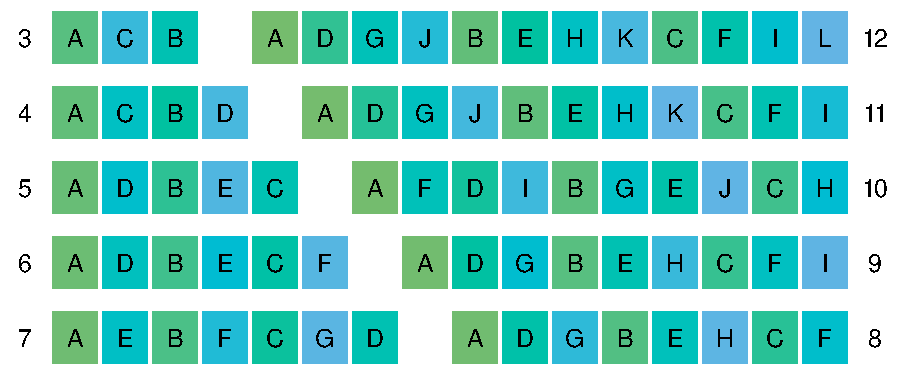
\includegraphics[width=3.5in]{Permutations.pdf}
  \caption{Permutations of siblings.}\label{fig:perm}
\end{figure}

Furthermore, adjacent leaf nodes with a different parent should have dissimilar colors in order to differentiate between branches. Therefore, the permuted color ranges within even numbered branches are by default reversed (\texttt{rev=true}). This is needed because the first category is always mapped to the lowest hue value, and the last category to a higher hue value. In Figure~\ref{fig:perm}, category A has the most greenish color in all shown cases, while the last categories are cyan or blue. To reverse the hue ranges in an alternating way, so only the even-numbered, the hue distance between any two adjacent nodes with different parents will increase, and thus easier to tell apart. 

Note that the labeling in Figure~\ref{fig:wheel} shows that the assignment of colors is permuted and also reversed for even-numbered branches. The three top-layer hue ranges [0, 120], [120, 240], and [240, 360] are permuted and therefore assigned to A, C, and B respectively. Since branches A and C are odd-numbered, their hue ranges are permuted but not reversed. The permutations of these branches are [A.1, A.3, A.2, A.4], and [C.1, C.3, C.5, C.2, C.4]. Since branch B is odd-numbered, its hue ranges are not only permuted, but also reversed: [B.2, B.3, B.1].

The result of these permutations is that siblings are better discriminated in each subsequent 
hierarchical layer, which is illustrated in Figure~\ref{fig:graph}. For comparison, the permutation 
is turned off in the node-link diagrams shown in Figure~\ref{fig:graph_noperm}. In the left diagram, the hue values 
form a gradual hue circle with only small hue gaps between branches, which are caused by hue fraction $f$ (see Subsection~\ref{secf}). In the right diagram the even-numbered branches are reversed. The leaf nodes of branch B are now more distinct from the other leaf nodes. However, the distinction between branches of the second hierarchical layer is still less than with permutation enabled (Figure~\ref{fig:graph}).

\begin{figure}[!b]

  \centering
  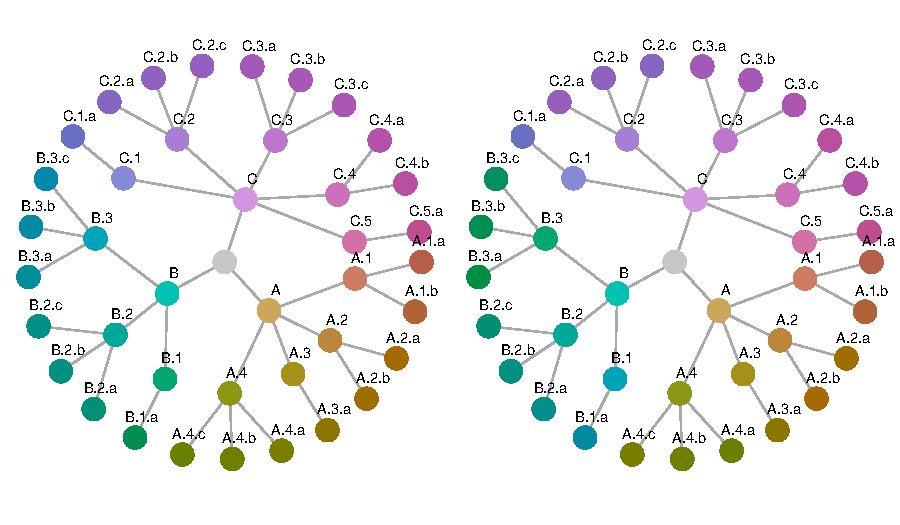
\includegraphics[width=3.5in]{HCPgraph2.pdf}
  \caption{Node-link diagrams with permutation disabled. Reversal of even-numbered branches is disabled on the left, and enabled on the right.}\label{fig:graph_noperm}

\end{figure}


The permutations and reversals of hue ranges is developed particularly for visualization methods in which sibling nodes are arranged linearly or radially. However, when sibling nodes are arranged differently, for instance in treemaps, adjacent sibling nodes might get indistinguishable colors.

\subsubsection{Hue fraction}\label{secf}

The fraction $f$ is needed to introduce a `hue gap' between nodes with a different parent. This choice is a trade-off between discriminating different main branches and discriminating different leaf nodes. If $f=0$, the hue ranges are diminished to single hue points, which implies that each main branch is assigned a constant hue. On the other end of the extreme, if $f=1$, the full hue range is available at each hierarchical layer, which makes leaf nodes easier to distinguish, but harder to take apart leaf nodes of different branches. However for a radial or linear layout this can be alleviated by using permutation and reversal.

\begin{figure}[tb]
  \centering
  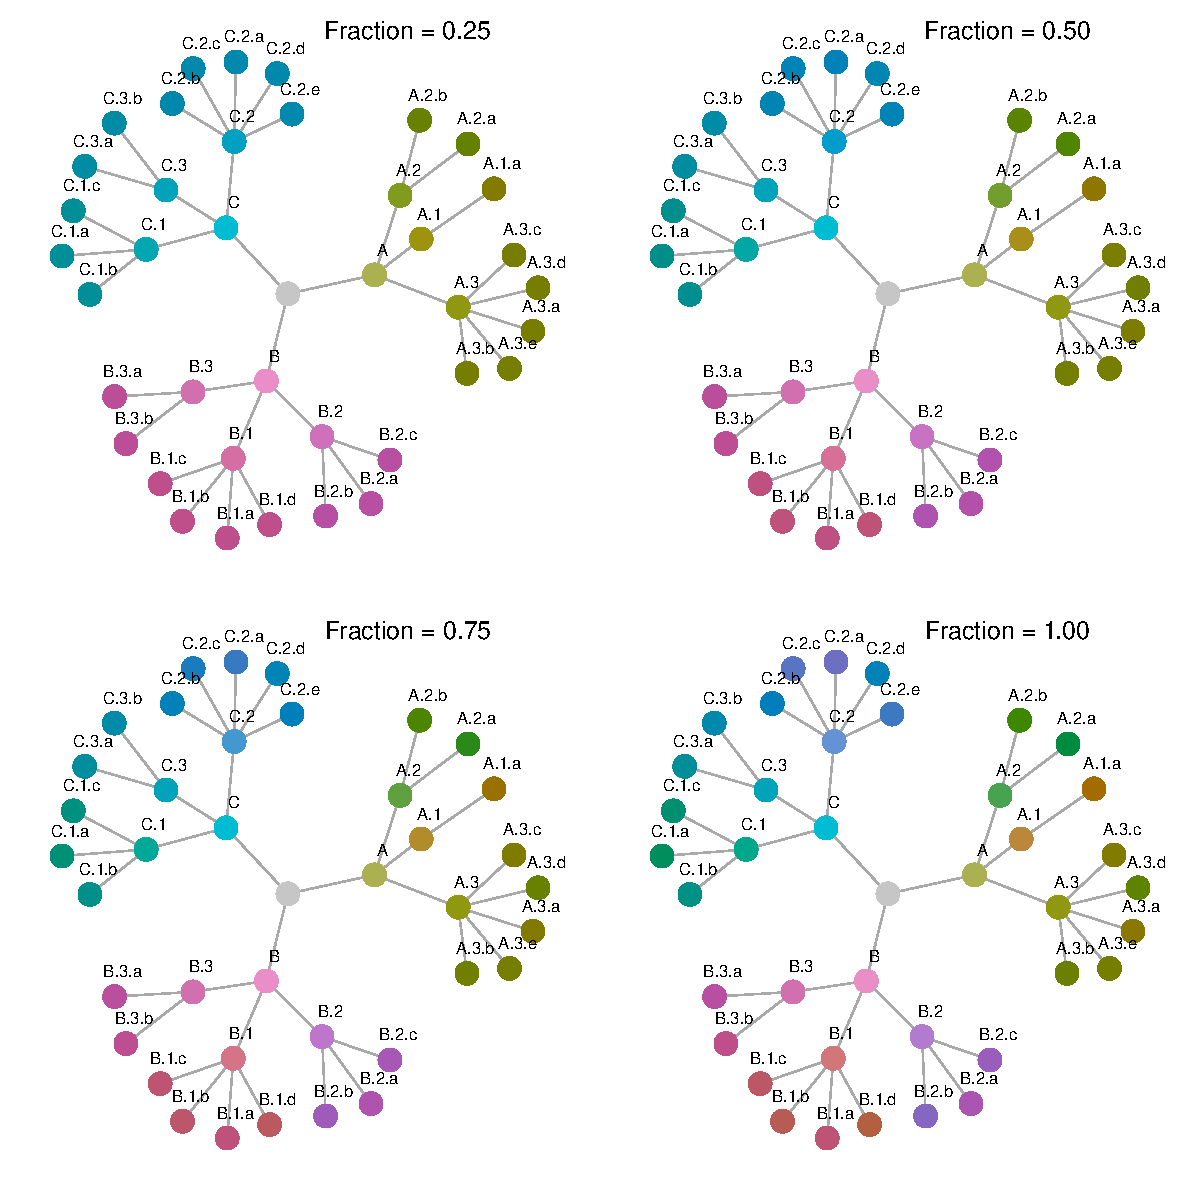
\includegraphics[width=3.5in]{Graph_hue.pdf}
  \caption{Node-link diagram with different fraction values.}\label{fig:graphf}
\end{figure}

The choice of $f$ depends on several aspects, such as the application, the size and dimensions of the hierarchical data, and on the used visualization method. In Figures~\ref{fig:graphf} a node-link diagram with a Fruchterman-Reingold layout~\cite{Fruchterman91} is shown with different values of ${f}$. For such explicit tree visualizations, high values of ${f}$ can be chosen to discriminate the leaf nodes without loosing tough of the global tree structure which is clearly visible, also without Tree Colors. Even values of (or close to) $1.00$ are appropriate here. To be on the save side, we suggest $f=0.75$ for explicit tree visualizations as a guideline.

\begin{figure}[!b]
  \centering
  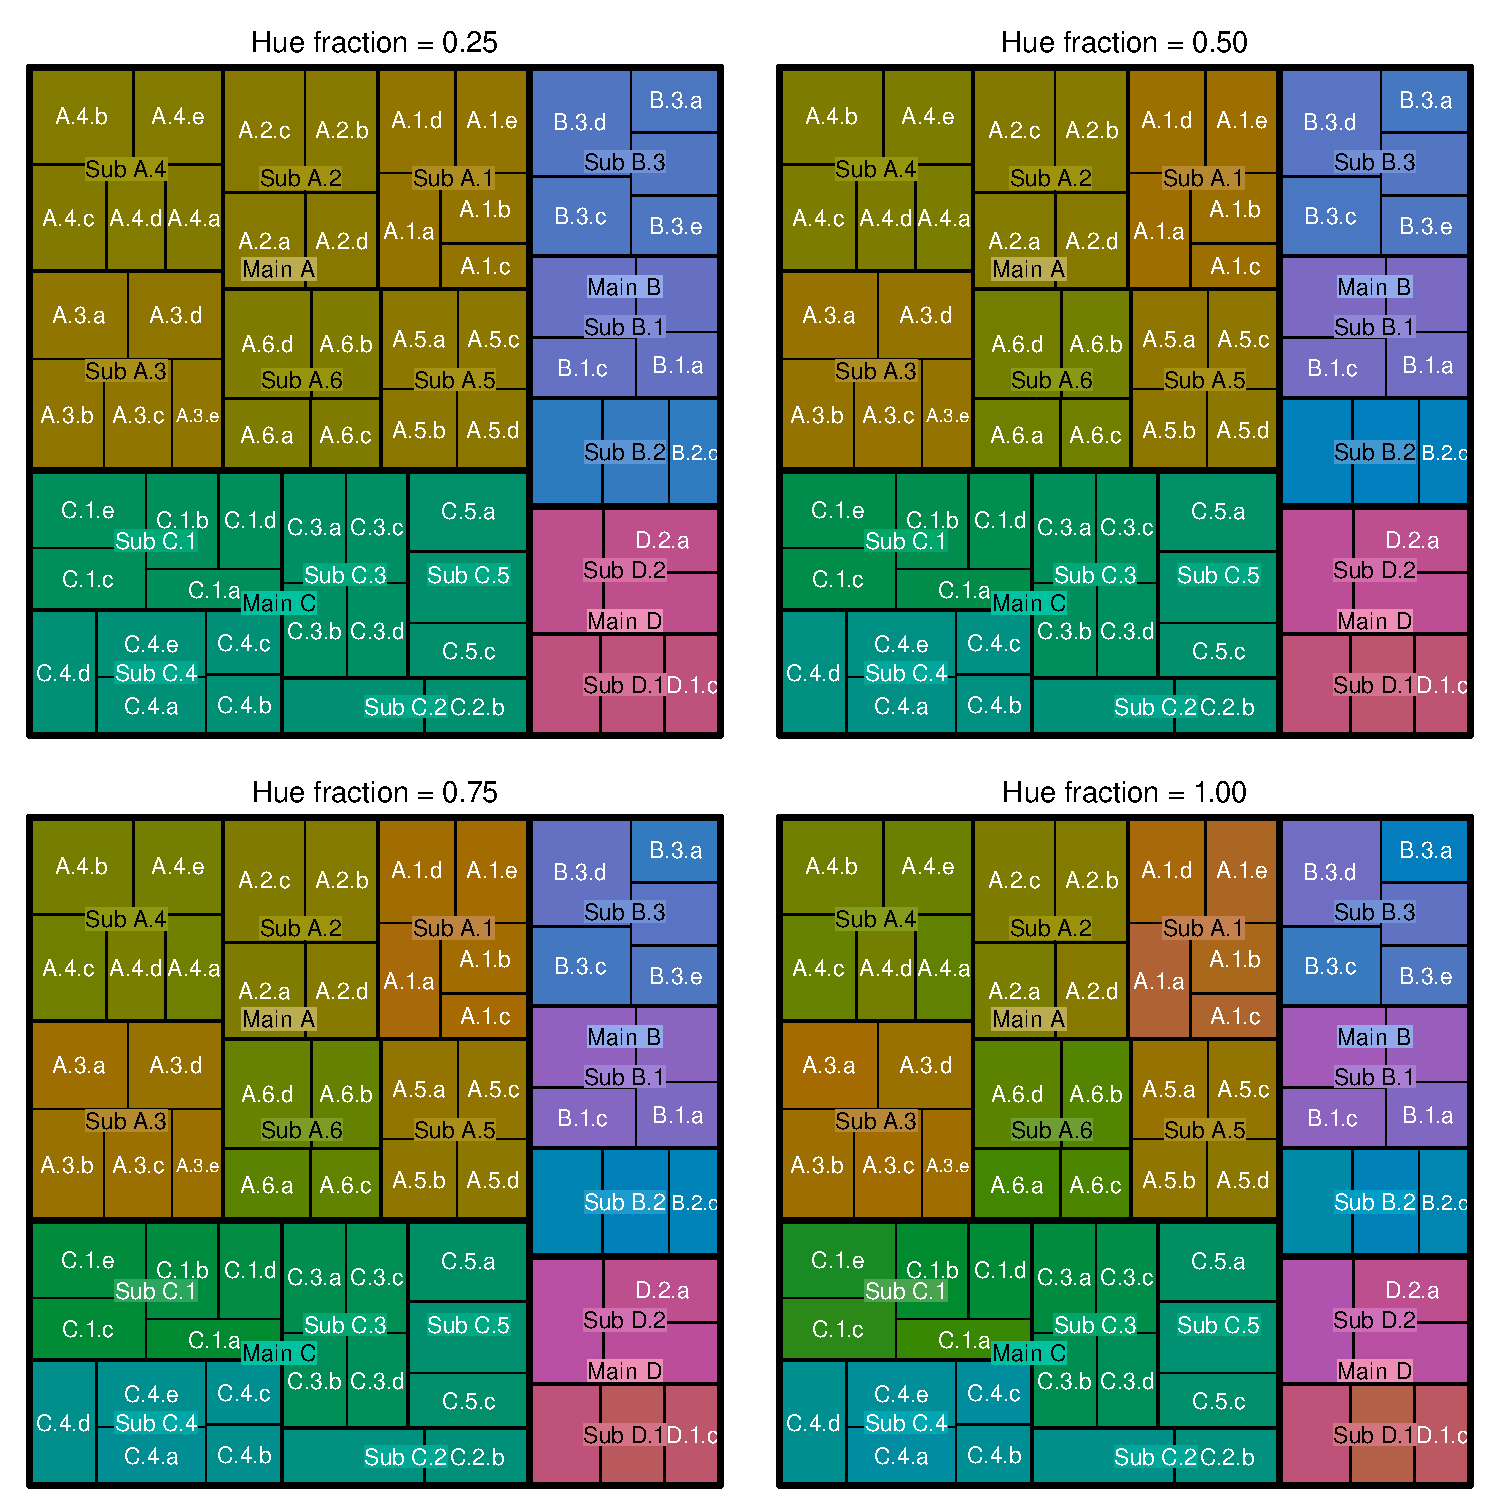
\includegraphics[width=3.5in]{Treemaps_hue.pdf}
  \caption{Treemaps with different fraction values.}\label{fig:treemapf}
\end{figure}


For implicit tree visualizations where the tree structure is not clearly visible without colors, lower values of $f$ are more suitable. This is illustrated with a treemap and different values of $f$ in Figure~\ref{fig:treemapf}. We applied the ordered treemap layout~\cite{Bederson2002} for these treemaps. For $f=0.75$ and especially $f=1.00$, it is difficult to quickly see the global tree structure; the main categories A and C are hard to take apart as well as the categories B and D. Therefore we suggest $f=0.50$ as a rule of thumb for implicit tree visualizations.

\subsection{Chroma and luminance values}

There are basically two methods to encode hierarchical depth in the colors of the nodes. Either brightness increases or decreases with depth. If brightness increases, leaf nodes will be brighter but also less saturated than nodes high in the tree. We refer to this method as the additive color method, since by metaphor, the leaf node colors can be seen as paint pigments that are mixed towards the dark gray root node. The other method is the subtractive color method in which leaf nodes can be seen as dimmed light beams that are mixed towards the light gray root node. Here, a child node is darker and little more saturated than its parent node.

Throughout this paper, we will use the subtractive color method by default, but the additive color method can be used just as well. The node-link diagram in Figure~\ref{fig:graph} illustrates the subtractive color method. The nodes in the first hierarchical layer, A, B, and C have the brightest colors which are a little less saturated than the other colors. In Figure~\ref{fig:graphadd} the same diagram is shown where the additive color method is applied. In this method A, B, and C are the darkest nodes (except for the root node), and also have the most saturated colors.

\begin{figure}[tb]
  \centering
  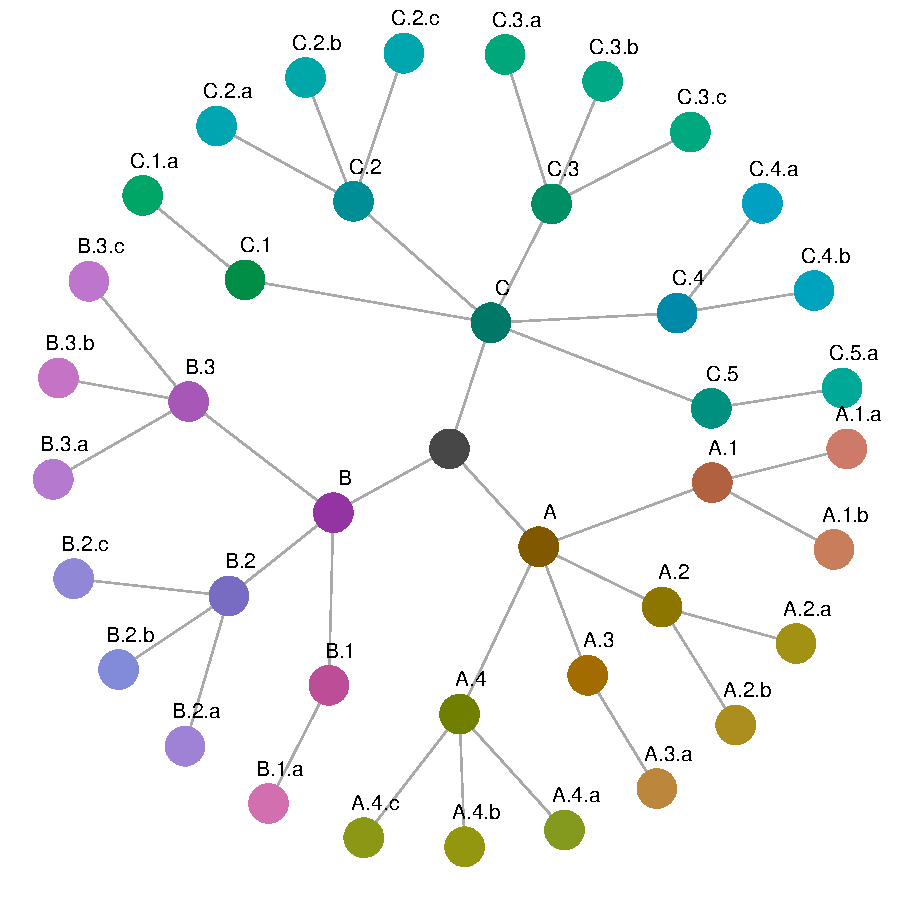
\includegraphics[width=3.2in]{HCPgraph3.pdf}
  \caption{The additive color method.}\label{fig:graphadd}
\end{figure}


For the subtractive method, we let luminance decrease linearly with depth. We set the default luminance value for the first (highest) layer below the root as $L_1=70$. For the other layers $i=2,\ldots, d$, where $d$ is the depth of the tree, the luminance value is defined as
\begin{equation}
L_i=(i-1)\beta^L + L_1,
\end{equation}
where the default value for the slope parameter $\beta^L$ is set to $-10$. In case the root node is visualized, it is colored gray. Its luminance value is specified by $L_0=L_1-\beta^L$. For the additive method, in which luminance increases with depth, we suggest $L_1=40$ and $\beta^L=10$. 

\begin{figure}[tb]
  \centering
  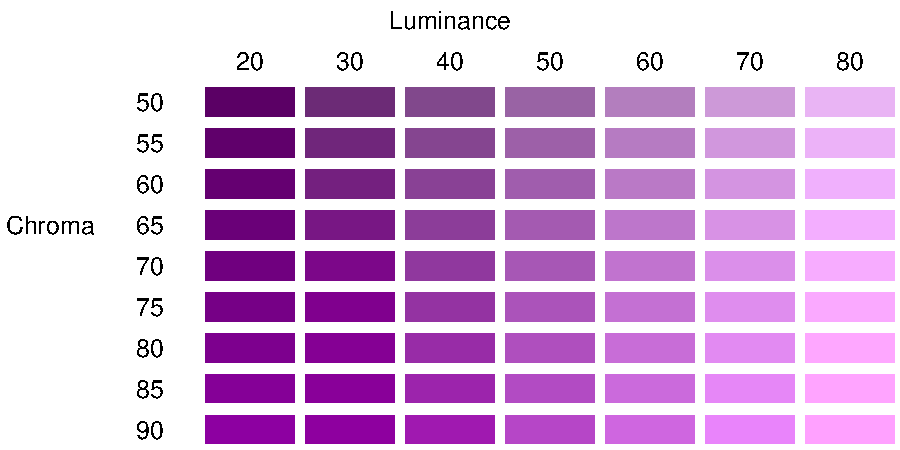
\includegraphics[width=3.5in]{LC.pdf}
  \caption{Colors for different $L$ and $C$ values with a constant $H=300$.}\label{fig:lc}
\end{figure}

In Figure~\ref{fig:lc} a table of colors are depicted for various chroma and luminance values and a constant hue of $H=300$. Brighter colors (with higher values of $L$) have the tendency to become too saturated in our opinion, for instance, the colors with $L=70$ and $C\geq70$. However, for dark colors, high values of $C$ may help to discriminate them distinguish them from other dark colors with different hue values. The question therefore is, what values of $C$ are needed for what values of $L$ in order to distinguish the colors easily without using too much saturation.


\begin{figure}[!b]
  \centering
  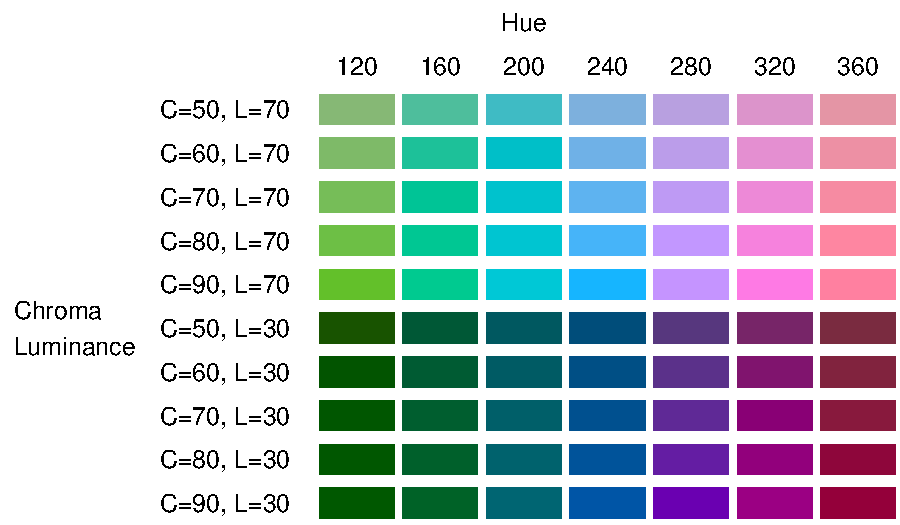
\includegraphics[width=3.5in]{LC2.pdf}
  \caption{Colors schemes for different pairs of $L$ and $C$.}\label{fig:lc2}
\end{figure}

For different pairs of $C$ and $L$, color schemes with a fixed hue range from 120 and 360 are depicted in Figure~\ref{fig:lc2}. Among the bright color schemes (with $L=70$), the saturation level of $C=60$ is sufficient to discriminate the colors easily. For the dark color schemes (with $L=30$), saturation values of $C=80$ or higher are not superfluous, especially because the assigned hue range is often very narrow for nodes low in the tree.

Therefore, we propose to increase $C$ with depth for the subtractive color method. Let $C_1=60$ be the chroma value for the first layer. For layer $i=2,\ldots, d$ the chroma value is defined as
\begin{equation}
C_i=(i-1)\beta^C + C_1,
\end{equation}
where the slope parameter is set to $\beta^C=5$ by default. The chroma value for the root node is irrelevant, since it is colored gray. Chroma decreases with depth in the additive method. For this we suggest $C_1=75$ and $\beta^C=-5$.

So per hierarchical layer $i$, we have specified a fixed pair of $L_i$ and $C_i$ based on the parameters $L_1$, $\beta^L$, $C_1$, and $\beta^C$. For the default values of these parameters using the subtractive color method, we depicted the pairs with a fixed hue values between 120 and 360 in Figure~\ref{fig:lc3}. The pairs for the additive method are by default identical, but reversed where the parameter values for first layer are $C_1=75$ and $L_1=40$.

Although we propose default parameter values for luminance and chroma, the choice of these values depends on the number of hierarchical layers in the data, and on which layer the attention is focused. The default parameter values for the subtractive method provide colors that are well distinguishable within the first three layers. Therefore, they are particularly useful for datasets up to three hierarchical layers. However, when only leaf nodes of the third layer are visualized, such as in treemaps of data that have a complete tree structure of depth three, a higher $L_1$ value may be preferred. Also, when the dataset contains five of more layers a higher value of $L_1$ may also be preferred. In these cases, we suggest $L_1$ to be 80 or even 90. In order to prevent colors that become too saturated, we suggest $C_1$ to be 55 or 50 in this situation. However, when more discrimination among the colors is needed, higher values of $C_1$ may be chosen.

\begin{figure}[!t]
  \centering
  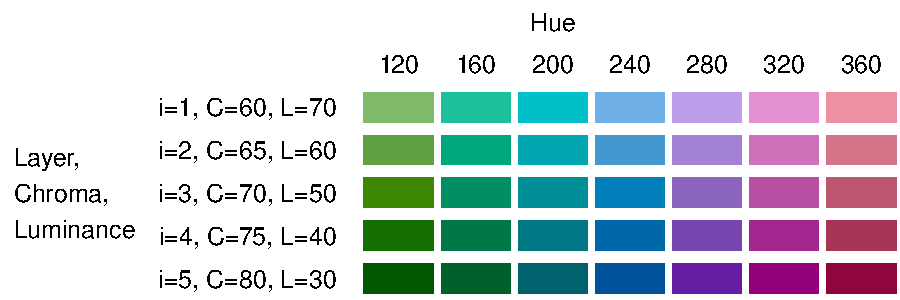
\includegraphics[width=3.5in]{LC3.pdf}
  \caption{Colors schemes for matched pairs of default $L$ and $C$ values for the top five hierarchical layers.}\label{fig:lc3}
\end{figure}



\subsection{Parameter overview}

An overview of all parameters that are used in the described method is provided in Table~\ref{table:param}. The abbreviations sub and add stand for subtractive respectively additive color method.

Due to the ranges of $[0, 100]$, the luminance and chroma parameters are restricted to the following constraints:
\begin{equation}
0 \leq (d-1)\beta^L + L_1 \leq 100
\end{equation}
and 
\begin{equation}
0 \leq (d-1)\beta^C + C_1 \leq 100.
\end{equation}

Notice that hue values are radial degrees where 360 degrees is a full circle. In order to rotate the hue range, we also allow negative numbers. Furthermore, it is also possible to set $H_{end} < H_{start}$. In that case, the direction in which hue values are assigned is counter-clockwise instead of clockwise.

\begin{table}[!htb]
\begin{footnotesize}
\begin{center}
\begin{tabular}{lllll}
\toprule
\multicolumn{2}{l}{Parameter    } & Range & \multicolumn{2}{l}{Default value} \\
\midrule
Hue start 				& $H_{start}$ &-360 to 360  & \multicolumn{2}{l}{0}      \\
Hue end   				& $H_{end}$ & -360 to 360 & \multicolumn{2}{l}{360}       \\
Hue fraction 				& $f$	& 0 to 1 & \multicolumn{2}{l}{0.75 (explicit)} \\
					&	&	 & \multicolumn{2}{l}{0.50 (implicit)} \\
Hue permutations 			& \texttt{perm} & boolean & \multicolumn{2}{l}{TRUE}      \\
Hue reverse   			& \texttt{rev} & boolean  & \multicolumn{2}{l}{TRUE}    \\
\cmidrule(r){4-5}
					&		&		& Sub. & Add. \\
\cmidrule(r){4-5}
Luminance first level value 	& $L_1$	& 0 to 100  & 70 & 40      \\
Luminance slope value 		& $\beta^L$ &       & -10  & 10      \\
Chroma first level value 		& $C_1$ &  0 to 100  & 60   & 75    \\
Chroma slope value 		& $\beta^C$ &     & 5   & -5    \\
\bottomrule
\end{tabular}
\end{center}
\end{footnotesize}
\caption{Parameters of the Tree Colors method.}\label{table:param}
\end{table}

\subsection{Color vision deficiency}
Although Tree Colors were not developed with color blindness in mind, it is important to know whether Tree Colors are 
perceived adequately by people with a color vision deficiency, because that is quite common~\cite{birch12}.

People with normal color vision, called trichromates, perceive colors by three classes of cone opsins, the S-, M-, 
and L-cone opsins, that have absorption peaks at short (bluish), medium (greenish),  respectively long (reddish) wavelengths. Colorblind people only have two classes of cone opsins, and are therefore called dichromats. It may also occur that people have all three classes of cone opsins, but that the absorption peaks of two of them are shifted closer together than normal. Those people, called anomalous trichromats, are able to see the full color spectrum, but have difficulty distinguishing particular colors.

%Color vision deficiency is caused by the disfunctioning of one of the three type of cone cells by which people normally perceive colors. The three type of cone cells correspond one to one to the perception of the three primary colors red, green, and blue. People with normal color vision, trichromats, perceive any color as a mixture of the three types of cone cells, whereas people with a non-functional type of cone cell, dichromats, use a mixture of the two remaining types of cone cells to perceive colors. People with a partly disfunctional type of cone cell are called anomalous trichromats. They require more light of the corresponding primary color wavelength in order to perceive colors normally.

People with color vision deficiency cannot easily differentiate colors with different hue values. Especially distinction between reddish and greenish colors are often problematic for them. If this would be the only obstacle for them to use Tree Colors, a straightforward solution would be to adjust the Tree Colors method by omitting these problematic hue ranges. However, there is a more fundamental problem for people with color vision deficiency. Since the adaption of colors by cone opsins is approximately logarithmic rather than linear, dichromacy or anomalous trichromacy will result in losing the perceptual properties of the HCL color space. In other words, people with a color vision deficiency may not perceive colors with different hue values and constant luminance and chroma values as equally bright and saturated.

Figure~\ref{fig:colblind} shows how people with color vision deficiency would probably see the full hue cycle depicted in Figure~\ref{fig:wheel}(a). These simulated plots are created with free software tool Chrometric~\cite{chrometric}. The left-hand side plot shows how the full hue circle is seen by anomalous trichromats with deuteranomaly, the most common type of color vision deficiency, where colors of medium wavelength (greenish) colors are not perceived well. Although all hue values seem to be distinguishable, the colors do not seem to be perceived equally bright and saturated. The plot on the right-hand side is seen by dichromats with protanopia, where the long wavelength (reddish) colors are not perceived. Not only the diversity of hue values is reduced, the colors also have a large variation in brightness and saturation.

\begin{figure}[tb]
  \centering
 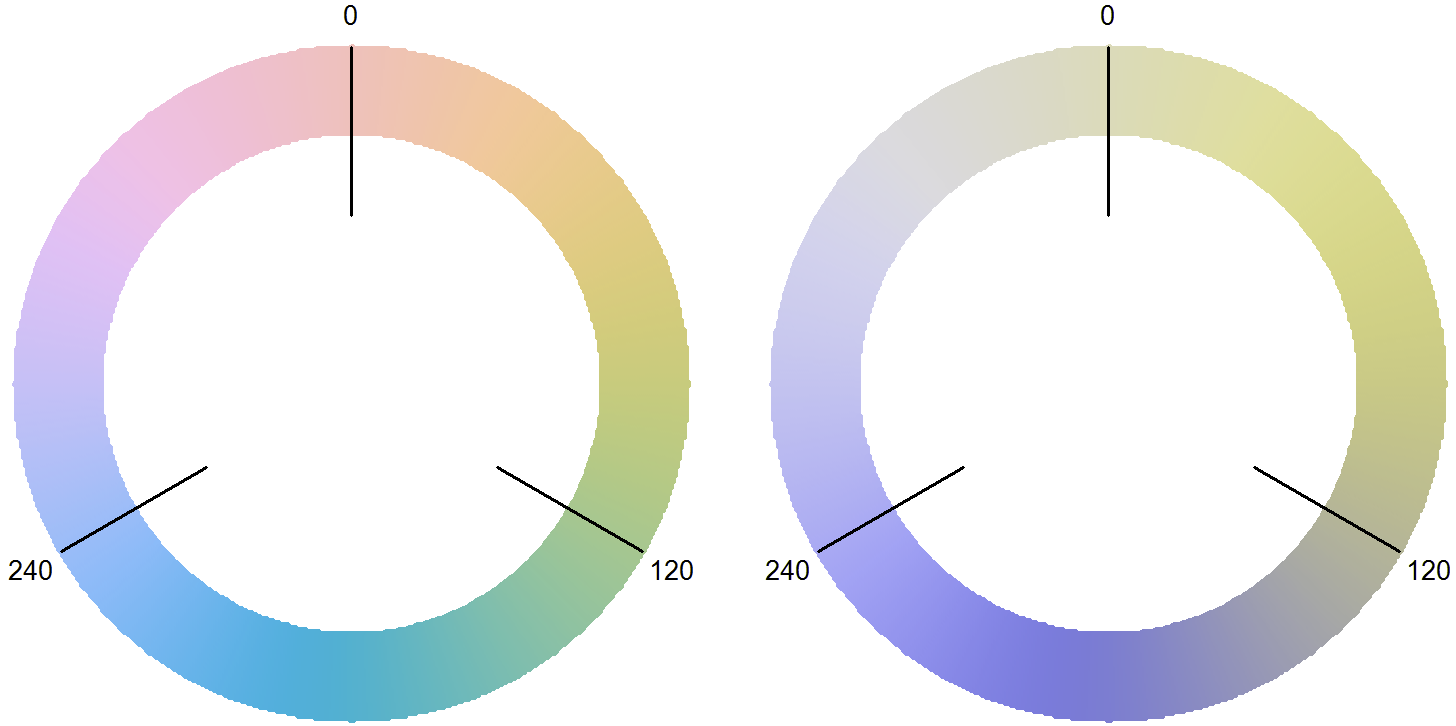
\includegraphics[width=3in]{hcl_deuteranomaly_protanopia.png}
  \caption{Simulation of how persons with deuteranomaly (left) and protanopia (right) see the full hue circle.}\label{fig:colblind}
\end{figure}


\section{Software}

The Tree Colors method is implemented in the \texttt{treemap} package~\cite{treemap} of the statistical software environment R~\cite{r2013}. All treemaps in this paper are created directly with this package, without post-processing. The implemented layout algorithms are the ordered treemap layout algorithm (pivot by size)~\cite{Bederson2002} and the squarified treemap layout algorithm~\cite{bruls99}. By default, Tree Colors are used to emphasize the hierarchical structure of the data. However, the color attribute can also be used for a second variable or to compare two hierarchical datasets~\cite{tennekes2011b}. The node-link diagrams in this paper are also created with the \texttt{treemap} package. The layout of the nodes are processed with the dependency package \texttt{igraph}~\cite{igraph}.

To visualize Tree Colors and to tune its parameters, the \texttt{treemap} package contains an interactive tool called \texttt{treecolors}. With this tool, users can create random tree structured data, and experiment with the parameters. Four visualizations can be shown: two node-link diagrams (Reingold-Tilford and Fruchterman-Reingold), a treemap and a bar chart. It also provides a table of the data that includes the color values in hexadecimal format and the HCL values of all tree nodes. The sunburst plot is generated with \texttt{d3.js}~\cite{bostock2012d3} and Tree Colors.

%\afterpage{\clearpage}


\section{Applications}\label{secapplication}

In this section, we discuss the application of Tree Colors to tree visualizations with real-world statistical data.

\subsection{Economic activity}

The \textit{Nomenclature statistique des activit\'es \'economiques dans la Communaut\'e europ\'eenne} (NACE)~\cite{nace} is a classification system of economic activicy that is often used for national statistics on business enterprises. In Figure~\ref{fig:graphFRApp}, the NACE labels of the sector G, wholesale and retail trade, are depicted by a node-link diagram with the Fruchterman-Reingold layout algortihm~\cite{Fruchterman91}. Other layout algorithms, e.g. Kamada-Kawai~\cite{Kamada89}, typically better express the tree structure but at the cost of having less space per node. Using Tree colors allows for a more spaced-out layout scheme by expressing tree structure in color.

%National statistics on business enterprises are often published per economic sector. Economic sectors are typically structured hierarchically. For instance, the class of bakeries may have a parent class food manufacturers, which in turn is a child of the class of manufacturers. All member states of the European Union use same classification system of economic activity, namely the \textit{Nomenclature statistique des activit\'es \'economiques dans la Communaut\'e europ\'eenne} (NACE) system~\cite{nace}. This system has 21 main economic sectors and consists of four hierarchical layers.

Figure~\ref{fig:sunburst} shows the net turnover of the Dutch wholesale and retail trade enterprises in 2011~\cite{cbsSBS} in a sunburst layout~\cite{stasko2000evaluation, stasko2000focus+} with Tree Colors. The angle of an arc corresponds to its net turnover. A sunburst plot, which is a radial version of a layered icicle plot~\cite{kruskal1983icicle,burch2010indented}, typically repeats the same qualitative color scheme for child nodes: sibling nodes have different colors, but their children use the same color scheme. This makes siblings more distinct, but makes the tree structure less visible. In contrast, Tree Colors better show the hierarchical structure of data.


In Figure~\ref{fig:treemapApp}, the same dataset is visualized by a treemap. The Tree Colors of the non-leaf nodes are used for the text label
 backgrounds. Notice that the colors of the third NACE layer nodes, for instance the pink colored 466, are brighter than the colors of the other leaf nodes. The depth of leaf nodes is more difficult to observe in treemaps than in other visualization methods such as a sunburst diagram, apart from the used color schemes.


% The number of digits in the category names represent the hierarchical layer. Each of the three main branches of this sector (45, 46 and 47) clearly has a distinct hue range. Furthermore, some leaf nodes, for instance the pink colored 466, are a brighter than others, because they represent the third rather than the fourth NACE layer.}

%Figure~\ref{fig:graphKKApp} shows the same diagram with a different layout using the Kamada-Kawai algorithm~\cite{Kamada89}. In comparison to the Figure~\ref{fig:graphFRApp}, the leaf nodes are more clustered in space by the Kamada-Kawai algorithm. This may clarify the tree structure better, but at the cost of possible artifacts. In this case there are two crossed edges, namely 465-4652 and 464-4643. The Tree Colors of the corresponding nodes help to discriminate the two local branches that overlap in layout.

\begin{figure}[t]
  \centering
  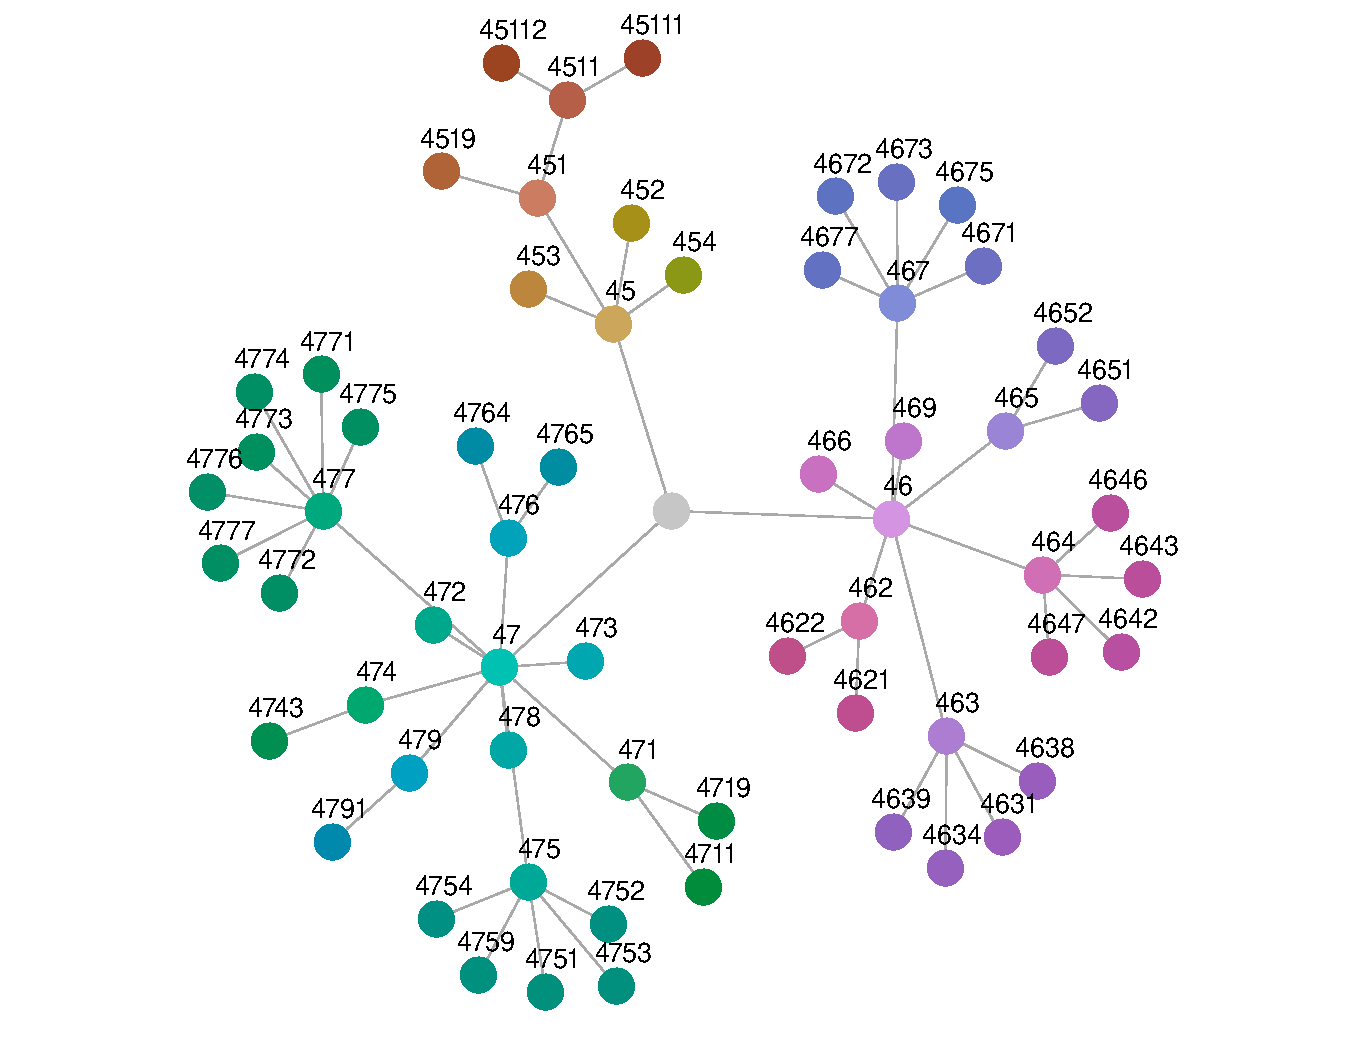
\includegraphics[width=3.5in]{Gbusiness_FR.pdf}
  \caption{Node-link diagram of all wholesale and retail trade NACE labels produced by the Fruchterman-Reingold layout algorithm.}\label{fig:graphFRApp}
\end{figure}


%\begin{figure}[!b]
%  \centering
%  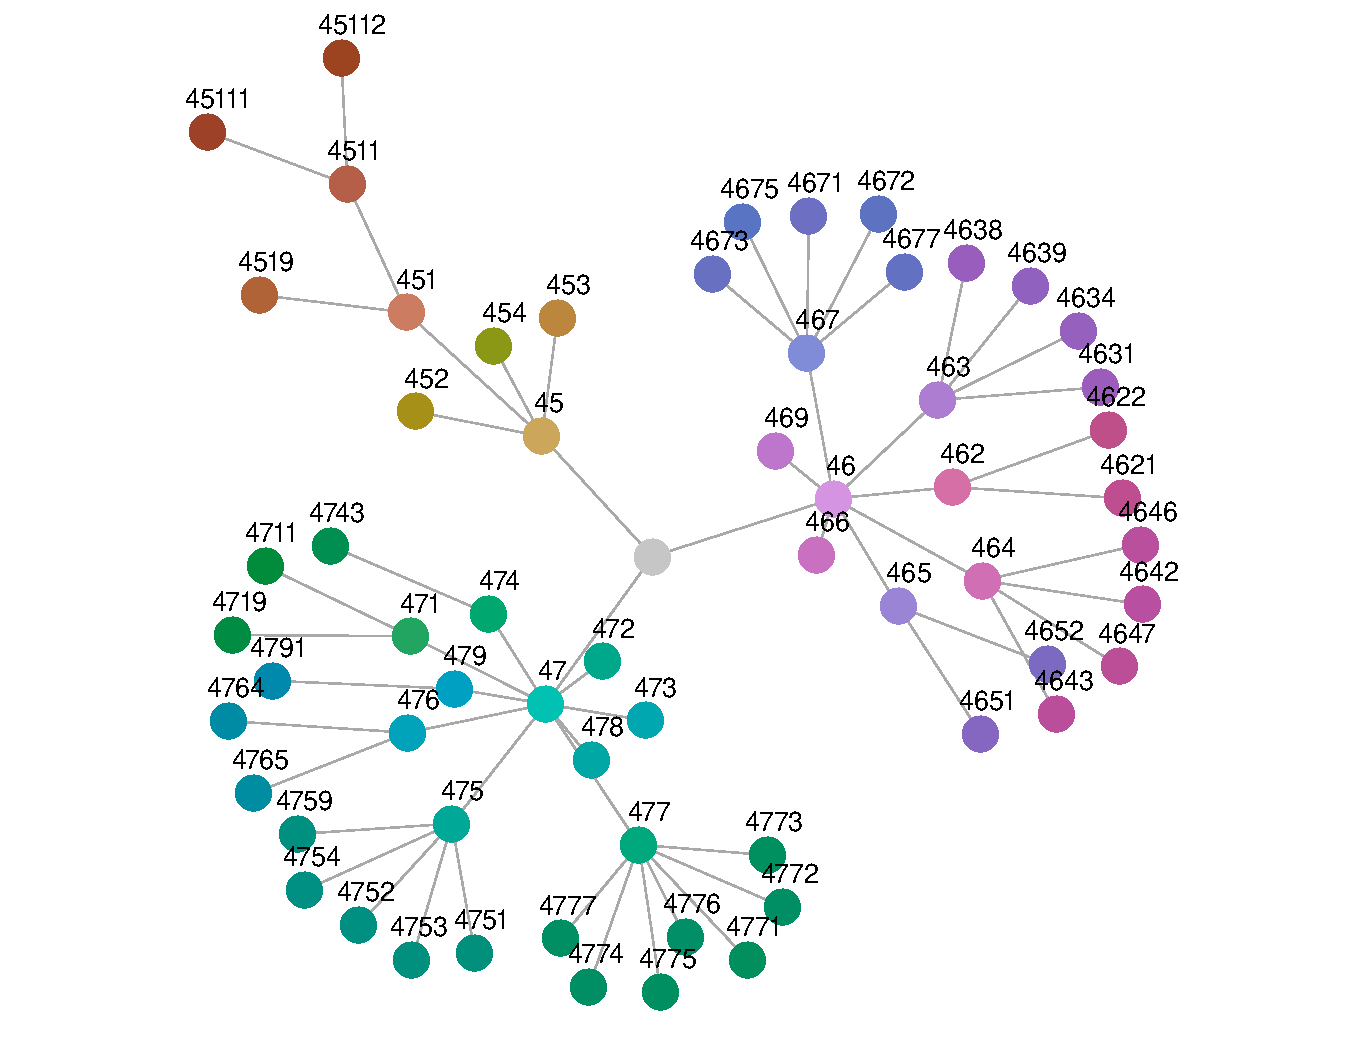
\includegraphics[width=3.5in]{Gbusiness_KK.pdf}
%  \caption{Node-link diagram of all wholesale and retail trade NACE labels produced by the Kamada-Kawai layout algorithm}\label{fig:graphKKApp}
%\end{figure}

\begin{figure}[!b]
  \centering
  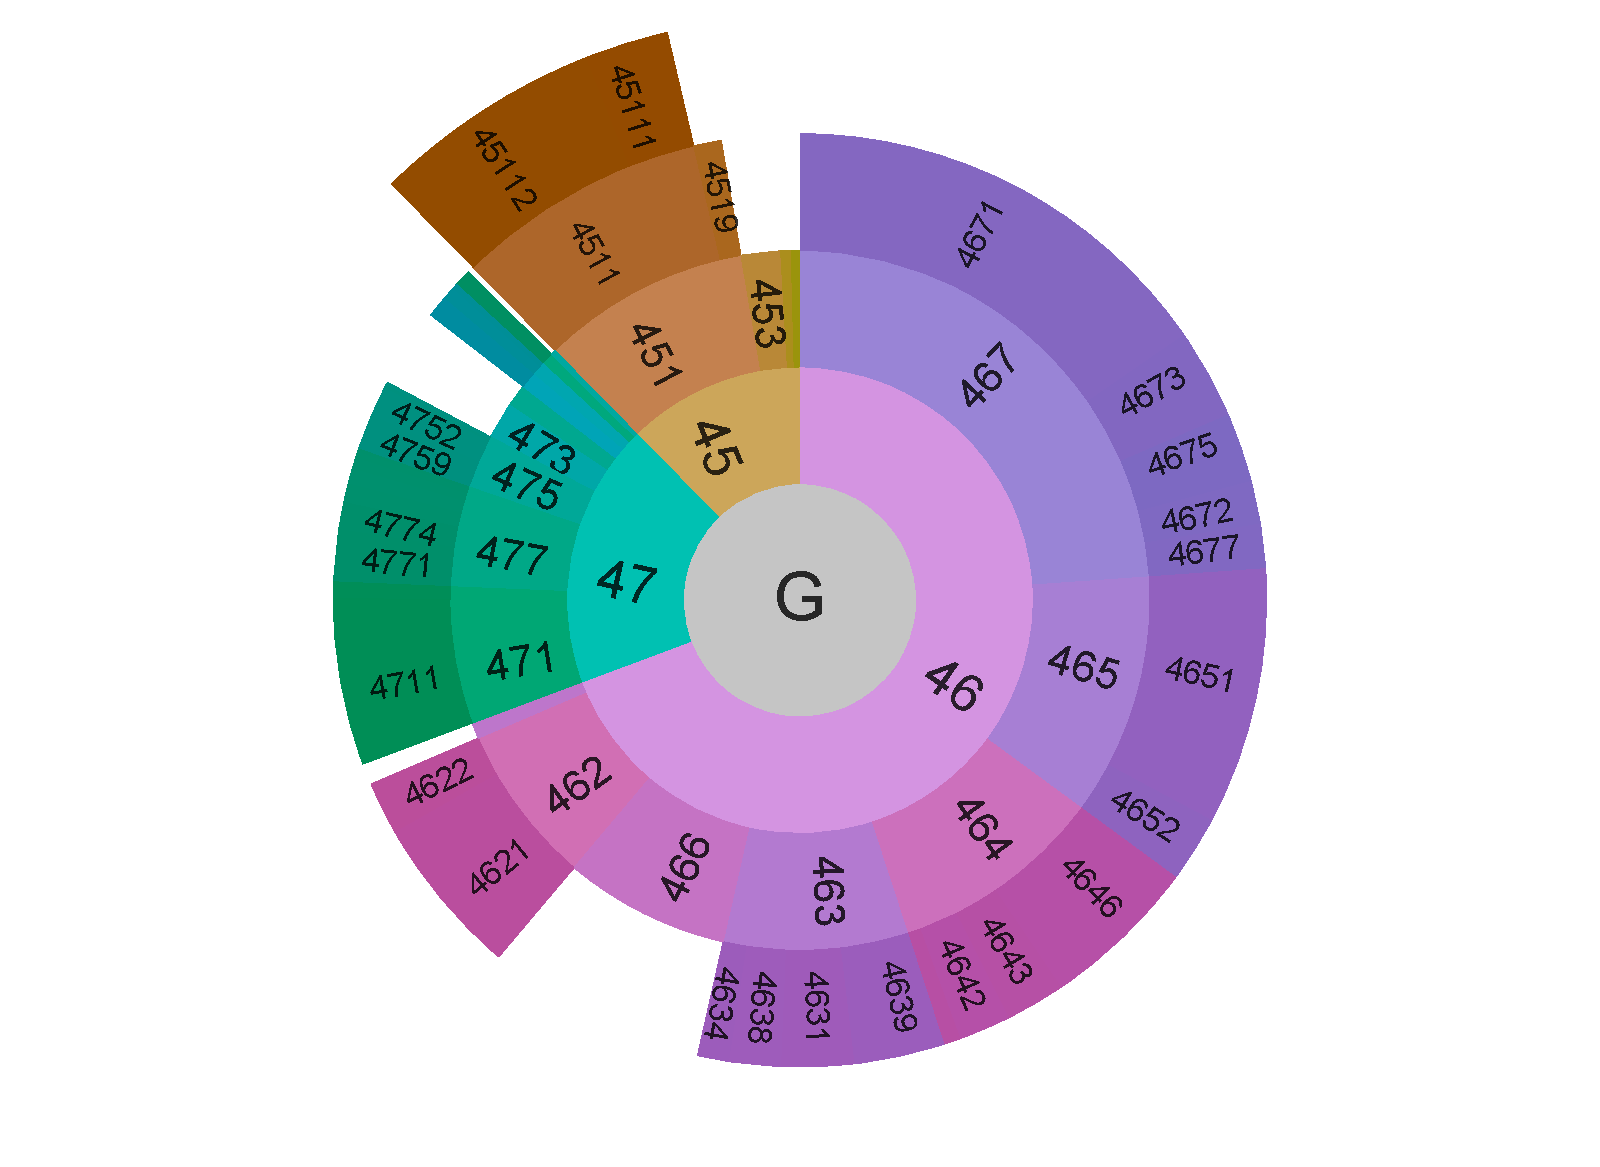
\includegraphics[width=3.5in]{sunburst/sunburst.pdf}
  \caption{Sunburst diagram with Tree Colors.}\label{fig:sunburst}
\end{figure}

%One of the largest European statistics that uses the NACE system are the Structural Business Statistics (SBS) that cover industry, construction, trade, and services. The main target variables are turnover, number of persons employed, total purchases, and financial result. These statistics are produced for the entire European Union. However, the applied production method which include data collection, editing, analyses and estimation may vary from country to country, depending on the budget, legislation, and the availability of administrative data sources such as tax data and the chamber of commerce. As for the Netherlands, data from small enterprises, i.e., less than 10 employees, are taken directly from tax administrations, data from medium enterprises (up to 50 employees) are taken from a sample survey, and data from large enterprises (50 employees or more) are taken from a full sample survey~\cite{cbsSBS}.

%In current practice, the SBS data are analysed separately per main economic sector, since for each sector domain specific knowledge is required.



\begin{figure}[!t]
  \centering
  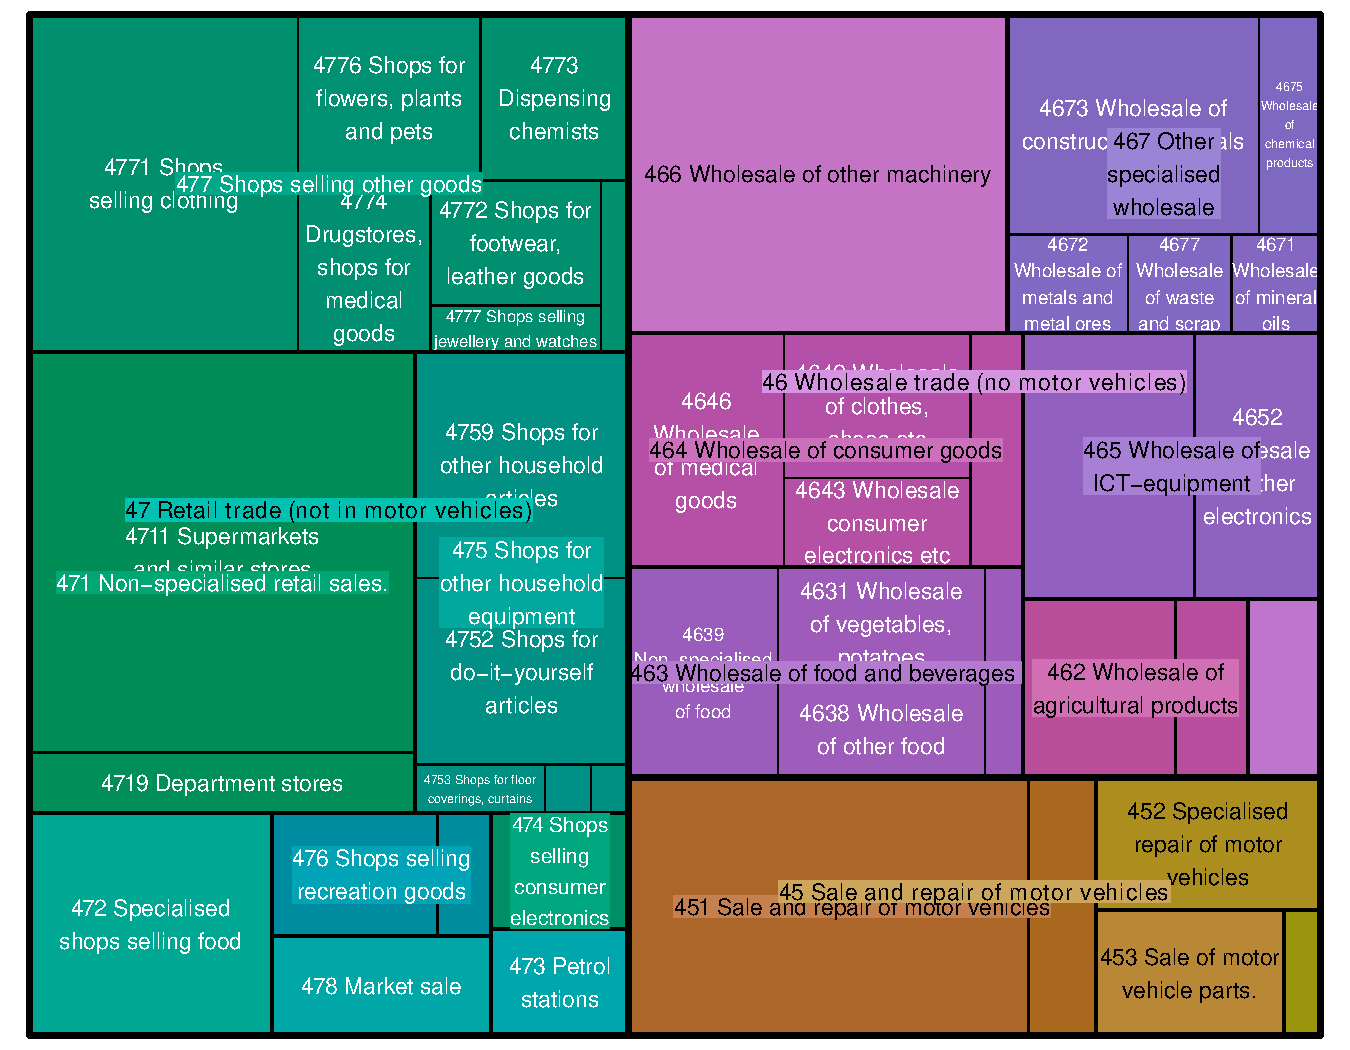
\includegraphics[width=3.5in]{TMbusiness.pdf}
  \caption{Turnover among Dutch wholesale and retail trade enterprises in 2011.}\label{fig:treemapApp}
\end{figure}

\subsection{Regional classifications}
Many publications in official statistics are broken down by region, especially regarding demographics.
In many situations, thematic maps are useful as a data visualization tool for spatial statistics, in particular choropleths and cartograms. However, non-cartographic methods are often sufficient for the task at hand. In those cases, the geographic location of the regions is less important for the analysis than the comparison of some specific target variable between regions. Tree Colors can improve the discrimination between the regions in a subtle way.

In Figure~\ref{fig:barApp} a bar chart, created with the R package ggplot2~\cite{ggplot2}, is shown of the Dutch population broken down by twelve provinces. For comparing the populations to each other, a bar chart is a good working horse, since length is perceived quite accurately~\cite{Mackinlay1986}. We applied Tree Colors to add information about the geographical layout of the provinces. Typically, the provinces are grouped by the cardinal directions north, east, west, and south. We use those directions as the first hierarchical layer, and the provinces themselves as the second hierarchical layer. The obtained Tree Colors discriminate the provinces while grouping them by cardinal direction. To enhance groupings, the vertical spaces between the cardinal directions are slightly increased.

\begin{figure}[!b]
  \centering
  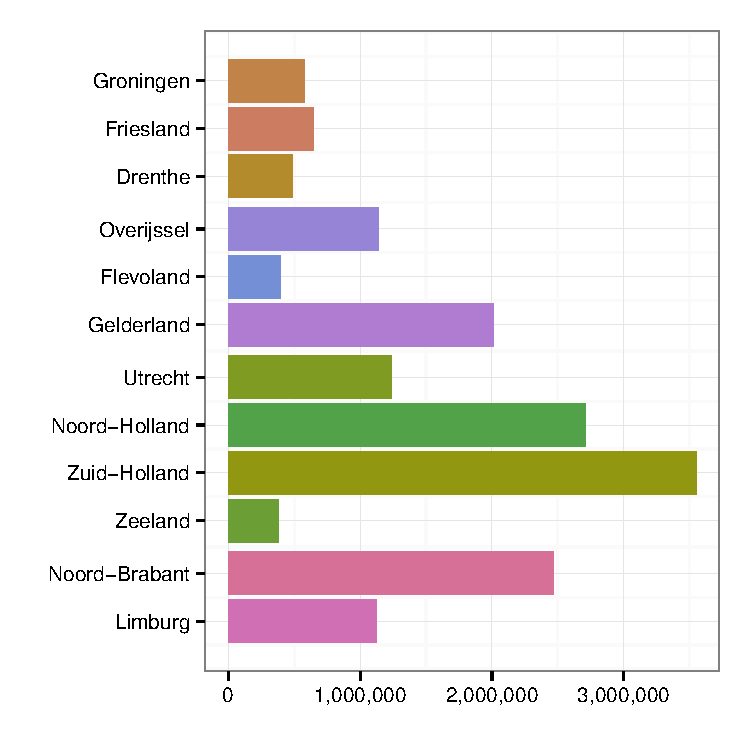
\includegraphics[width=3.5in]{pop_bar.pdf}

  \caption{Dutch population in 2012 per province.}\label{fig:barApp}

\end{figure}


\section{User study}~\label{secuser}
A user study has been conducted to evaluate our proposed method. We let participants compare Tree Colors to Main Branch Colors. Main Branch Colors form a qualitative color scale that assigns distinct qualitative colors to the children of the root and gives their offspring the same color as their parent. The colors are taken from the qualitative ColorBrewer color schemes~\cite{brewer03}, which are user tested and popular in cartography and statistical visualizations, and hence provide a good benchmark for Tree Colors. An alternative would have been testing
against a Tree Colors scheme with $f=0$, but such color schemes are not in common 
use and testing three colors schemes would have complicated the user study.

\subsection{Questionnaire setup}~\label{secusersetup}
The questionnaire was taken by employees of Statistics Netherlands. Although no specific 
demographic characteristics were asked, the participants typically have at least a bachelor's degree in 
quantitative sciences. Furthermore all employees are aged from 18 to 65 years old, and gender is 
approximately equally divided. In order to know whether 
a participant has a color vision deficiency, we directly asked the participants 
whether they are (partially) color blind. Participants who did no know the answer
to that question were tested for 
color vision deficiency using the Ishihara test~\cite{ishihara}. 

Three visualization methods were used in the questionnaire, namely the node-link diagram, the treemap, and the bar chart. For each of the three methods, participants received questions for two charts of two different datasets, one with Tree Colors and one with Main Branch Colors. 

\begin{figure}[tb]
  \centering
  \mbox{\subfigure{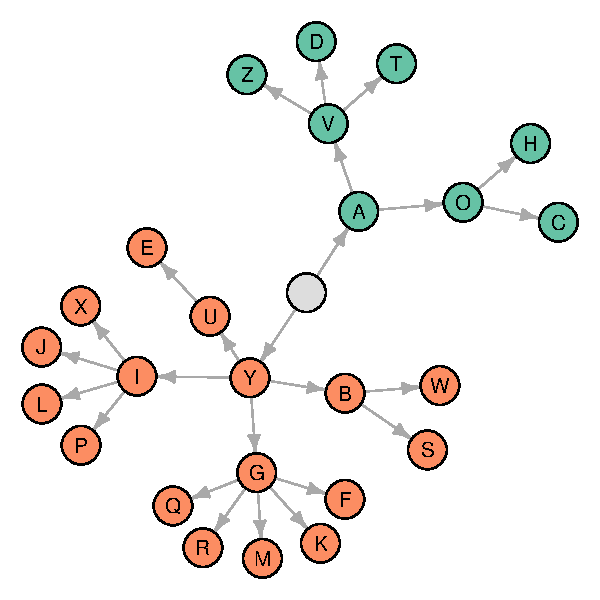
\includegraphics[width=1.7in]{Graph_survey_FC.pdf}}
  \subfigure{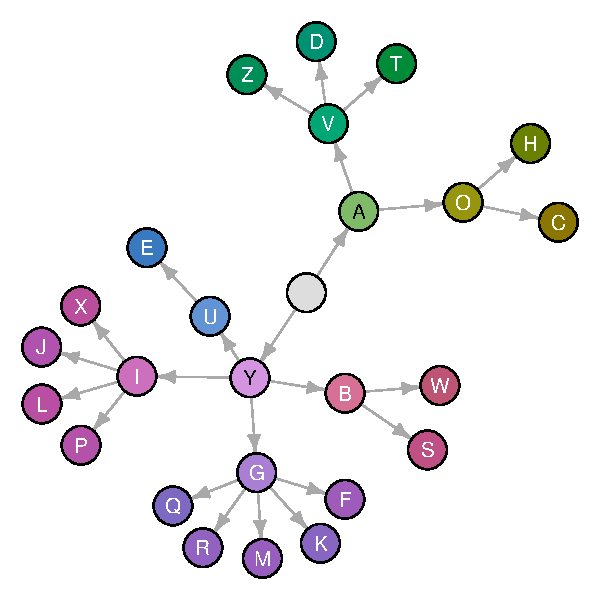
\includegraphics[width=1.7in]{Graph_survey_TC.pdf}}}
  \caption{Node link diagrams applied to Dataset 1 with Main Branch Colors (left) and Tree Colors (right).}\label{fig:graphSvy}

\end{figure}

In order to exclude the effects of all other aesthetics but color as much as possible, we distributed two different versions of the questionnaire. Each participant was randomly assigned to one version. For the two versions, the datasets for the Main Branch Colors and Tree Colors questions were swapped. Therefore, each chart was tested with both color schemes but in different groups. A node-link diagram, a treemap, and a bar chart that were included in the questionnaires are depicted in Figure~\ref{fig:graphSvy},~\ref{fig:treemapSvy}, and~\ref{fig:barSvy} respectively. An overview of the charts used in the two versions of the questionnaire is provided in Table~\ref{table:ques}. We alternated the used color schemes per visualization method in order to prevent a repeating systematic pattern in the questionnaire. Unfortunately, it was not possible to invert the alternating schemes, since this would require two extra versions of the questionnaire.

\begin{table}[!htb]
\begin{footnotesize}
\begin{center}
\begin{tabular}{llll}
\toprule
Method & Color scheme & Version 1 & Version 2\\
\midrule
Node-link diagram & Main Branch Colors & Dataset 1 & Dataset 2\\
Node-link diagram & Tree Colors & Dataset 2 & Dataset 1\\
Treemap & Main Branch Colors & Dataset 4 & Dataset 3\\
Treemap & Tree Colors & Dataset 3 & Dataset 4\\
Bar chart & Main Branch Colors & Dataset 5 & Dataset 6\\
Bar chart & Tree Colors & Dataset 6 & Dataset 5\\
\bottomrule
\end{tabular}
\end{center}
\end{footnotesize}
\caption{Overview of charts in the questionnaire.}\label{table:ques}
\end{table}

 
The three visualization methods represent three levels of hierarchical explicitness. The node-link diagram clearly is an explicit tree visualization by the layout of the nodes and by the edges, which are depicted as directed arcs pointed from the root node. The treemap is an implicit visualization method, in which the hierarchical structure is less clear in comparison to the node-link diagram. Except \changedE{for} %from
color, the hierarchical structure is represented by the nesting of the rectangles, the thickness of the rectangle lines, and by the label fonts. The bar chart is in essence a non-hierarchical visualization method. However, the bar charts that were included in the questionnaire contained beside color an extra subtle hierarchical element in the spacing between the bars. The bars represent the leaf nodes of the tree structure and the amount of spacing between two bars is determined by the degree of relationship.

\begin{figure}[tb]
  \centering
  % 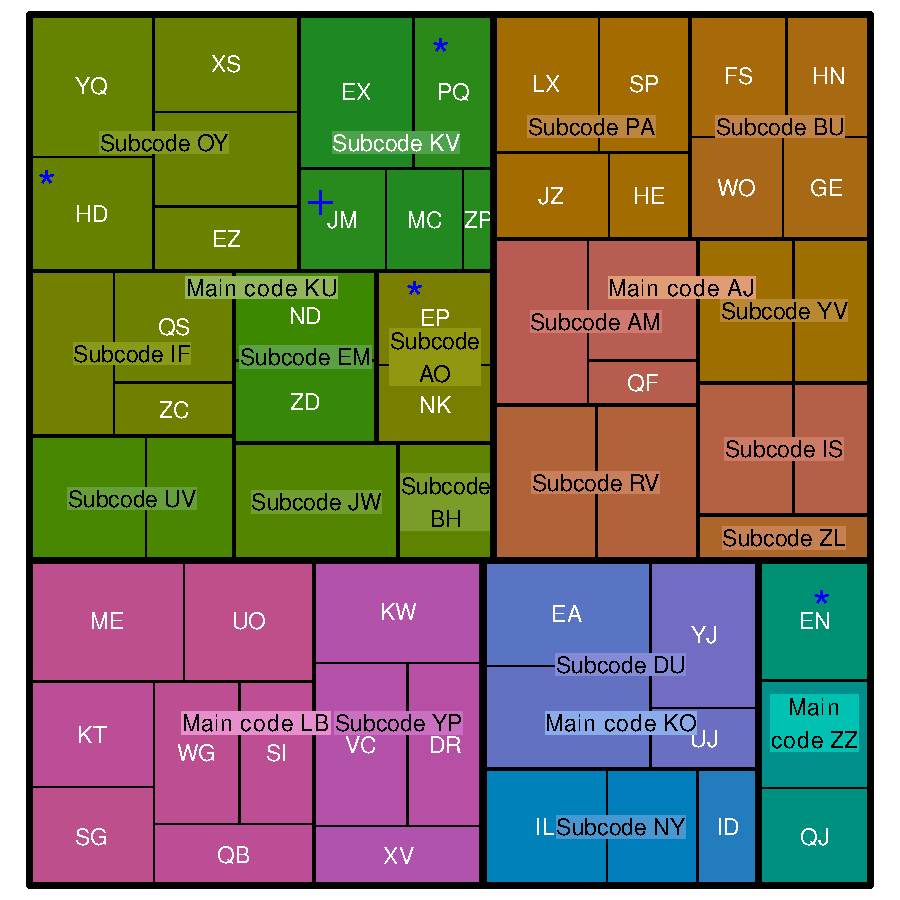
\includegraphics[width=3in]{Treemap_survey_TC.pdf}
  \mbox{\subfigure{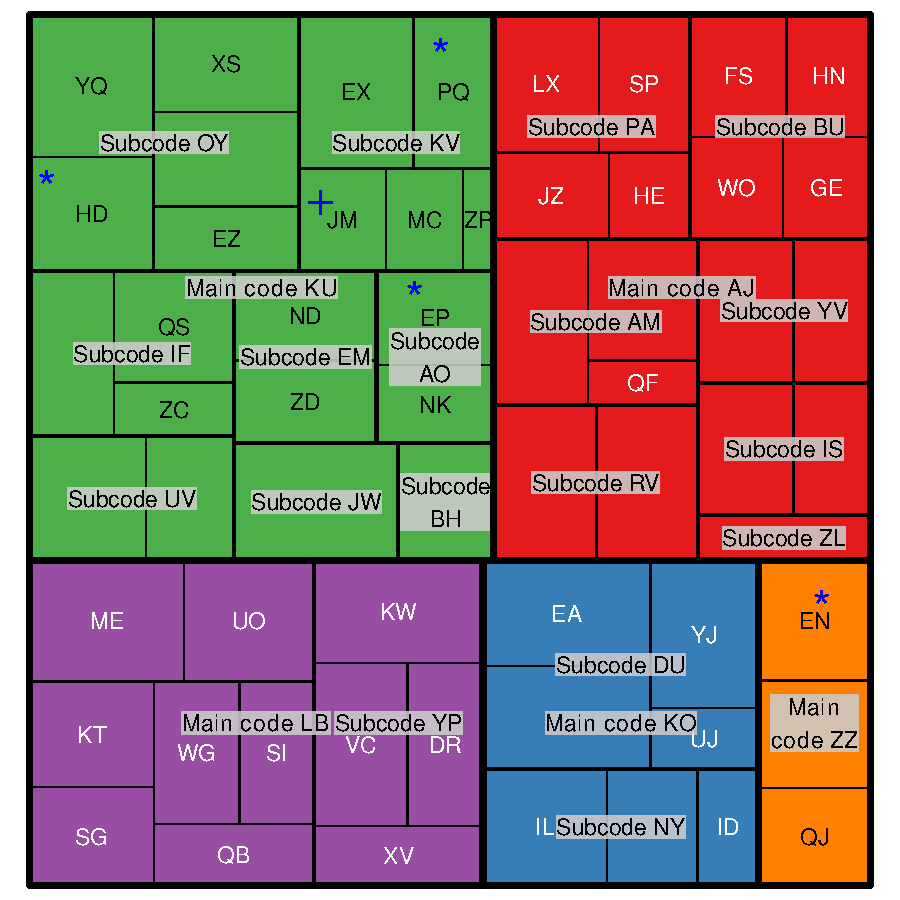
\includegraphics[width=1.4in]{Treemap_survey_FC.pdf}}
  \subfigure{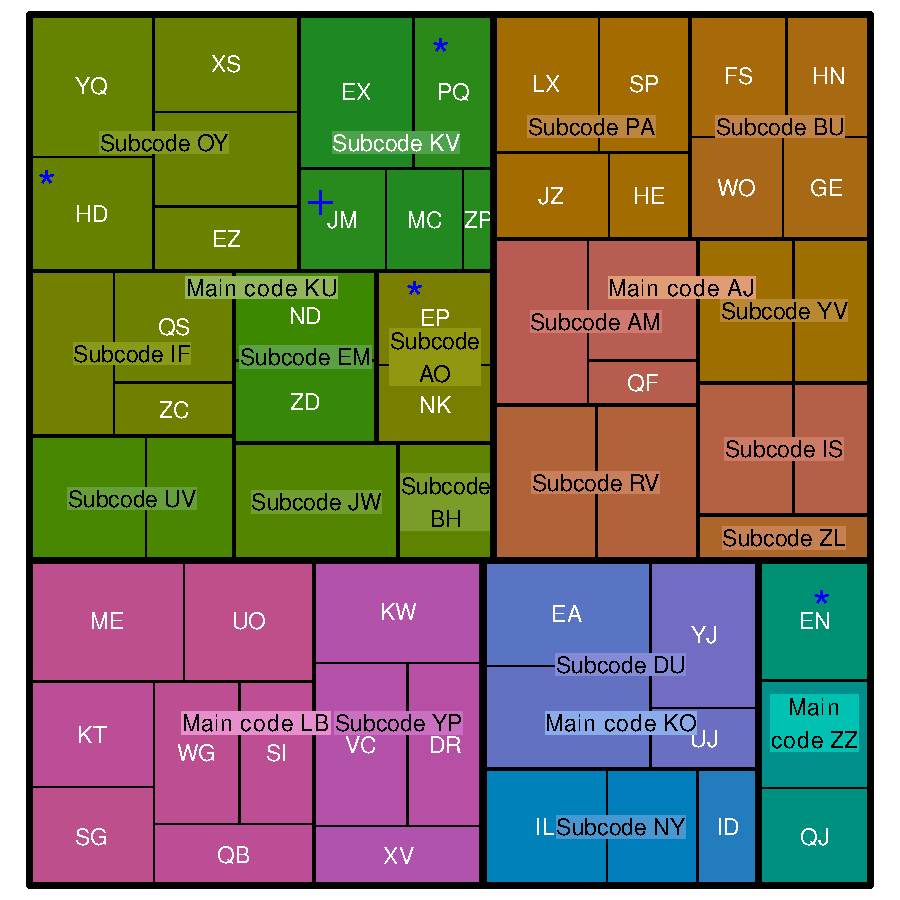
\includegraphics[width=1.4in]{Treemap_survey_TC.pdf}}}
  \caption{Treemaps applied to Dataset 4 with Main Branch Colors (left) and Tree Colors (right).}\label{fig:treemapSvy}

\end{figure}



\begin{figure}[tb]
  \centering
  \mbox{\subfigure{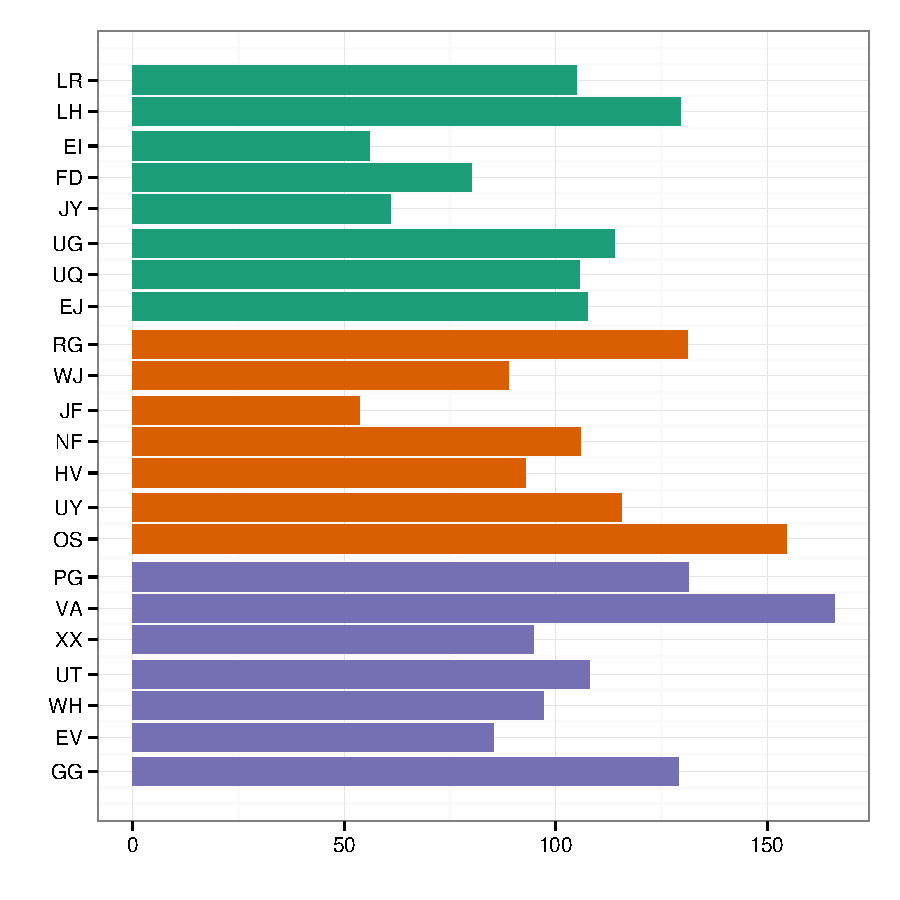
\includegraphics[width=1.7in]{Bar_survey_FC.pdf}}
  \subfigure{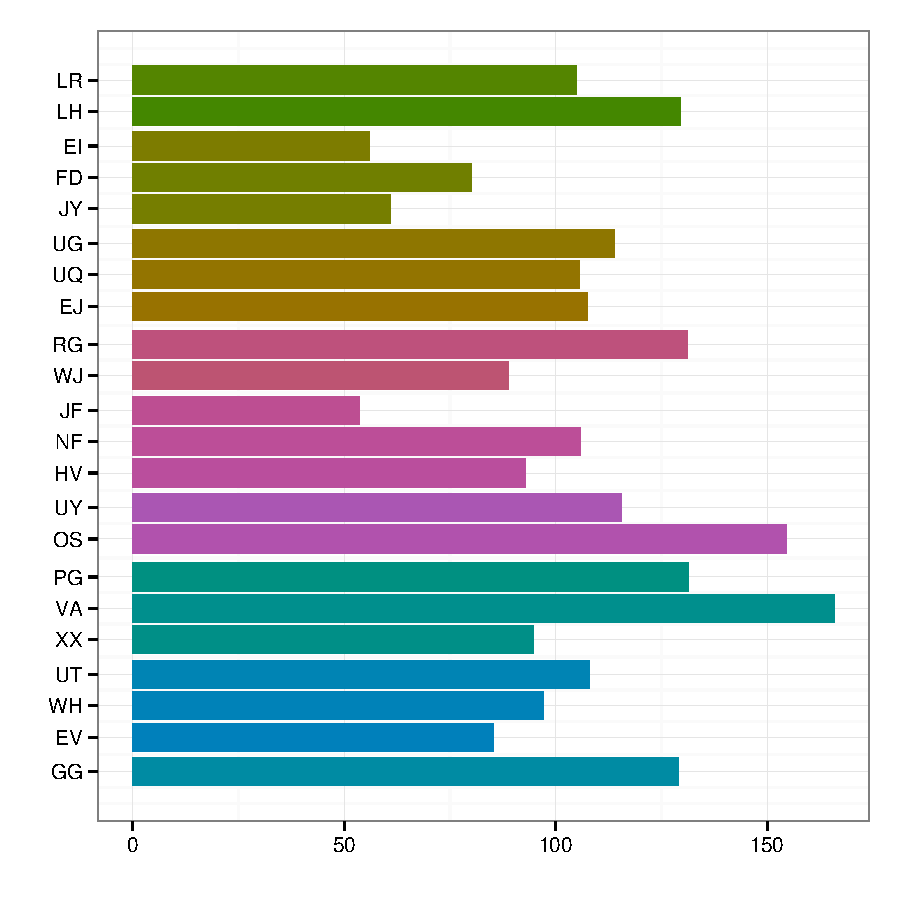
\includegraphics[width=1.7in]{Bar_survey_TC.pdf}}}
  \caption{Bar charts applied to Dataset 5 with Main Branch Colors (left) and Tree Colors (right).}\label{fig:barSvy}

\end{figure}

All datasets used in the questionnaire are hierarchically structured with three hierarchical layers. The 
labels of the data points are randomized letters, such that participants were not able to extract information 
about the hierarchy from the printed labels.

The questionnaire contained reading and evaluation questions. Per chart, participants got one or two reading questions and one evaluation question:
\begin{description}
\item[Relations] Which label(s) are most similar to X? The answer options consisted of one label from a different main branch than X, one or two labels from the same main branch but a different sub branch, and one label from the same sub branch as X. From the data structure point of view, we considered the last label as the correct answer.
\item[Offspring] How many sub-labels does main branch X have? This was an open question.
\item[Help] What do you think of the following statement? The charts colors helped me to answer the question(s) above. This question is a five-level Likert item with the answer options Strongly disagree (SD), Disagree (D), Neutral (N), Agree (A), and Strongly agree (SA).
\end{description}
Per visualization method, participants where asked those reading questions for two plots of different datasets, one with Main Branch Colors and one with Tree Colors. 
Next, participants were asked to evaluate these two plots with three questions:
\begin{description}
\item[Prettiness] Which chart is the prettiest?
\item[Interpretation] Which colors contributed most in interpreting the charts?
\item[Overview] Which colors provided the best overview?
\end{description}
Finally, participants were given the possibility to write down comments or suggestions.

\subsection{User study results}~\label{secuserres}

We recruited 98 participants with normal color vision and 10 participants with a color vision deficiency. From the people with normal color vision, 58 participants received Version 1 of the questionnaire and 40 Version 2. Among those with a color vision deficiency, 4 participants received Version 1 and 6 participants Version 2.

The results of the reading questions are summarized in the left part of Figure~\ref{fig:user1}. Per dataset the percentages of correct answers, that is, from a data structure point of view, are shown in orange for the Main Branch Colors and in blue for the Tree Colors. For each percentage, the corresponding $95\%$ confidence interval is depicted as a line. The right part of Figure~\ref{fig:user1} shows per visualization method the distribution of answers to the question whether colors had helped in answering the reading questions.

Of all three visualization methods, the reading questions regarding the node-link diagrams received the highest percentages of correct answers for both color schemes. The reason is the questions were fairly easy to answer by the explicit tree layouts of the node-link diagrams. 
The percentages of correct answers to the relationship question were a little higher with Tree Colors, although not statistically significant. The questions about the offspring resulted in 100\% scores. As for the node-link diagrams, participants experienced more help from Tree Colors than from Main Branch Colors.

The percentages of correct answers for the treemaps were lower than for the node-link diagrams. One reason could be that people are not familiar with treemaps; it turned out the many participants also took into account other aesthetics of the rectangles, in particular aspect ratio and area size, for answering the questions. Although the percentages of correct answers between both color schemes are comparable, the Main Branch Colors scored almost significantly better than the Tree Colors on the questions about the number of sub-labels for Dataset 4. This could be caused by the limitation that hue permutations and reversals were not designed for two-dimensional visualization methods. For treemaps, two adjacent rectangles may therefore get indistinguishable hue values, such as sub-labels PA and BU in the top-right corner of the treemap depicted in Figure~\ref{fig:treemapSvy} (left).


%The Tree Colors scored better the Main Branch Colors on the relationship question for Dataset 3. However, the scores on this question were identical for Dataset 4. This difference may be caused by the different color scheme instances that were applied. The Main Branch Colors scored better than the Tree Colors on the questions about the number of sub-labels. A possible explanation of this result could be that participants clustered the sub-labels colors by hue. For instance, for Figure~\ref{fig:treemapSvy} (left) participants were asked how many sub-labels Main label AJ has. The correct answer is 7, while one out of four participants thought the correct answer is 5. Probably, participants considered sub-labels PA and BU to be part of a different main label than the other 5 sub-labels. The amount of help that participants got from the applied colors was similar for Tree Colors and Main Branch Colors.

As for the bar charts, the majority of the participants did not observe the underlying data hierarchy when the Main Branch Colors were applied. Apparently, the spacing between the bars did not stand out clearly in comparison to other aesthetics such as color and length. For example, the question that belongs to Figure~\ref{fig:barSvy} (left) was which labels are most similar to UT, where the answers options are NF, XX, EV, and GG. Almost 52\% of the participants chose the labels that belong to the same main branch, XX, EV and GG, and therefore only used color to answer the question. Another 28\% only used length to answer the question, since they answered NF. Only 3\% of the participants answered EV, which is, given the data hierarchy, the correct answer. When Tree Colors were applied, see Figure~\ref{fig:barSvy} (right), none of the participants checked XX, EV, and GG, 23\% chose the equal-length bar NF, and 63\% answered EV correctly. This result indicates that Tree Colors can be a valuable attribute to visualize a hierarchical data structure in non-hierarchical plots such as bar charts, line charts, and area charts.


%By the broadly defined question, it would be a very weak argument to claim the success of Tree Colors on this large difference. However, in our opinion it does indicate that Tree Colors are a valuable attribute to visualize a hierarchical data structure in non-hierarchical plots such as bar charts, line charts, and area charts.

The three evaluation questions are summarized in Figure~\ref{fig:user2} with a diverging stacked bar chart. In general, the participants liked both color schemes equally, although Tree Colors were favored for node-link diagrams. Also, the participants found node-link diagrams with Tree Colors easier to interpret. The charts with Main Branch Colors provided the best overview for the majority of the participants. This result is not surprising, since a good overview is obtained by discriminating the main branches. Recall that Tree Colors can be adjusted with parameter $f$ in order to better discriminate main branches, and therefore getting a better overview at the expense of the discrimintaion of leaf nodes.

\begin{figure}[tb]
  \centering
	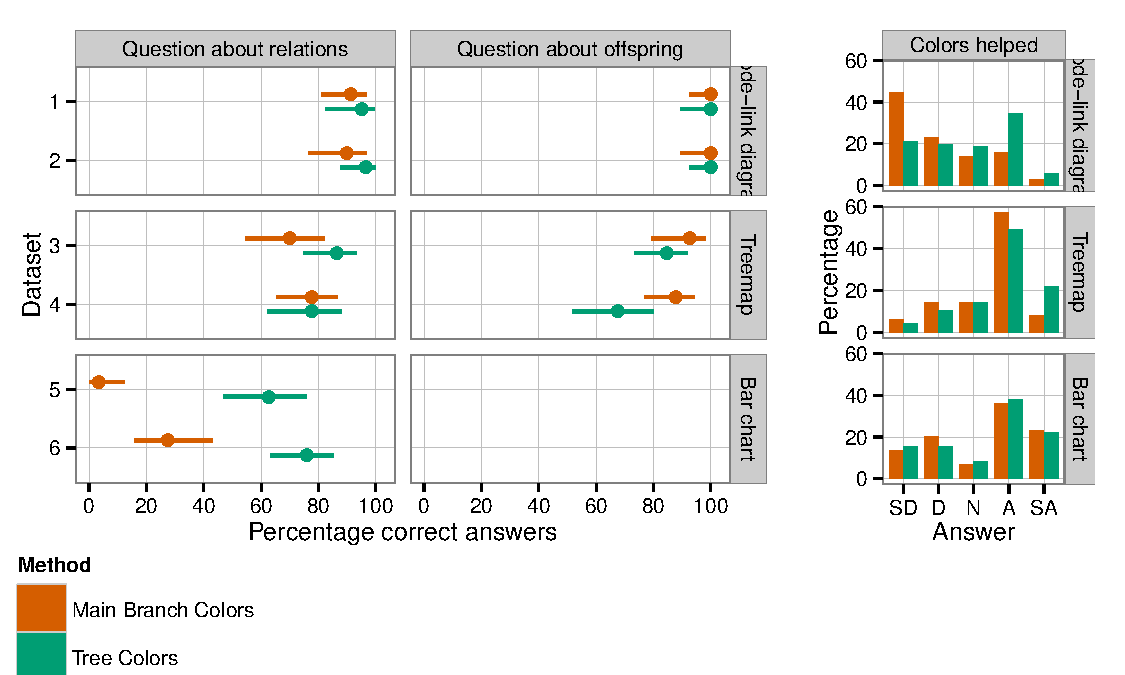
\includegraphics[width=3.5in]{user_study_results_mod2.pdf}
  \caption{Results of the reading questions.}\label{fig:user1}
\end{figure}


\begin{figure}[tb]
  \centering
	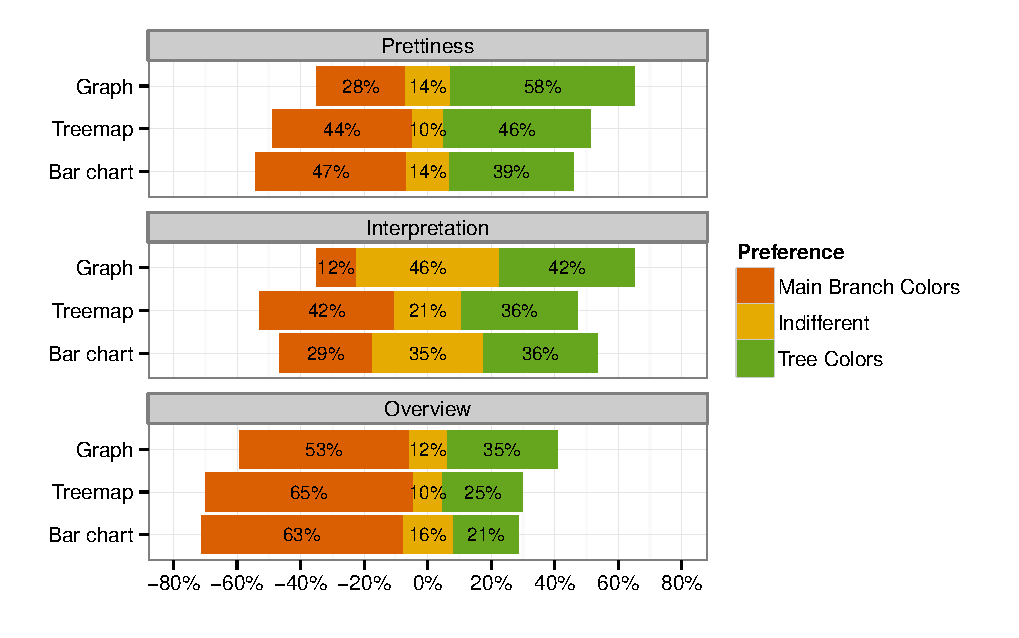
\includegraphics[width=3.5in]{user_study_results2.pdf}
  \caption{Results of the evaluation questions.}\label{fig:user2}
\end{figure}


%The interpretation of the node-link diagrams was experienced easier with Tree Colors except for the treemaps. This could be explained by level of difficulty of the visualization methods. Both node-link diagram and bar chart are easy to read visualization methods that the vast majority of the participants are familiar with. Therefore, people are able to see the benefits of the additional information that the Tree Colors provide over Main Branch Colors. However, treemaps are still largely unknown by the participants. Additional information provided by the applied color scheme could therefore be a little confusing.

The results of the user study regarding the 10 participants with color vision deficiency are summarized in Table~\ref{table:userCB}. By the small number of these participants, we were unable to make statistical claims from their responses. In line with the participants with normal color vision, most of them (64\%) experienced a better overview with Main Branch Colors than with Tree Colors (15\%).

\begin{table}[!htb]
\begin{footnotesize}
\begin{center}
\begin{tabular}{llllll}
\toprule
& \multicolumn{2}{l}{Node-link diagram} & \multicolumn{2}{l}{Treemap} & Bar chart\\
& relations & offspring & relations & offspring & relations\\
\midrule
M. B. C. & 7 & 10 & 5 & 10 & 0\\
Tree Colors & 7 & 10 & 5 & 6 & 3\\
\bottomrule
\end{tabular}
\end{center}
\end{footnotesize}
\caption{Numbers of correct answers to the reading questions asked to the 10 participants with color vision deficiency.}\label{table:userCB}
\end{table}

\section{Discussion}~\label{secdisc}

We proposed a method to create color schemes for tree structured data. In our opinion, this method improves both hierarchical and non-hierarchical visualizations methods when the tree structure of the data plays a role in the analysis. Tree Colors satisfy the three properties that we described in Section 1, namely that 1) all colors of a hierarchical color scheme should be unique, 2) the colors should reflect the tree structure in terms of parent-child relationships, and 3) hierarchical depth should be encoded in color. 

Although the choice to use hue to discriminate between different branches is straightforward and therefore not novel~\cite{yang2002, lam2012}, the actual mapping of tree structures to hue values involves two innovative techniques. First, we introduced hue gaps to obtain hue values that are grouped by branch to a certain extend, which is determined by the parameter $f$. The second novel technique is the permutation and reversals of the hue values, which results in a better differentiation of the nodes, both between siblings and between adjacent nodes with a different parent.

As for the hierarchical depth, we proposed a linear relation of depth with both luminance and chroma. By default we used the subtractive color method where luminance decreases and chroma increases with depth. The opposite holds for the additive color method that can be used alternatively. Further research on the preferences and usefulness of both methods is recommended.


For explicit tree visualizations such as node-link diagrams, the conducted user study suggests that Tree Colors \changedE{are} %can be 
a useful enhancement. Although most participants answered the questions regarding the node-link diagrams correctly for both color schemes, a large part of them found Tree Colors more helpful and found node-link diagrams with Tree Colors better to interpret than with Main Branch colors. As a consequence, using Tree Colors for node-link diagrams \changedE{enables relaxing} %could relax 
a hierarchical layout of the nodes, therefore spacing-out the placements of nodes and labels.

%The conducted user study in which Tree Colors are compared to standard qualitative color schemes, which we called Main Branch Colors, did not result in statistically significant differences. However, the user study provided some insightful results that could be useful for further research.

As mentioned in Section~\ref{sechueperm}. The coloring of sibling nodes is designed for layouts in which \changedE{they} are arranged linearly or radially. For two-dimensional visualization methods such as treemaps, two adjacent siblings can therefore get indistinguishable colors, which was also the case in the user study example. For further research, it is worthwhile to improve the permutation and reversal method for such visualization methods. Approaches to similar problems, such as the coloring of edges in a graph~\cite{Jianu09} may be useful.

More advanced user studies \changedE{might} %may 
reveal more insightful differences between Tree Colors and other tree coloring methods when applied to tree visualizations. 
It \changedE{may} %would 
be worthwhile to analyze response times~\cite{wang06} \changedE{to} %which could 
reveal differences between the effectiveness of both color schemes, and to conduct eye tracking experiments~\cite{burch11}, \changedE{to} %which could 
provide insight in how %well 
the participants understand the visualized tree structure with different color schemes.

We would like to remark that although the HCL color has well defined perceptual properties, the total range of hue values is not perceived perfectly linear, especially around non-primary colors. This could introduce certain artifacts in the resulting color schemes. For instance, the blue node U in Figure~\ref{fig:graphSvy} (right) seems to be more distinct from its parent Y than its siblings I, G, and B. Such artifacts could be overcome by rotating the total hue range with the parameters $H_{start}$ and $H_{end}$.

Unfortunately, Tree Colors are not adequately perceived by people with color vision deficiency, since the range of distinguishable hue values is reduced and colors with a constant luminance and chroma value may vary in perceived brightness and saturation. There are no straightforward solutions at hand to adjust the Tree Colors method for people with color vision deficiency Moreover, designing fixed qualitative color schemes for such people is already far from trivial~\cite{okabe02}. Further research is needed to develop hierarchical color schemes for people with color vision deficiency. From a practical point of view, we suggest to use color vision deficiency proof qualitative color schemes proposed in literature~\cite{okabe02, brewer03} as Main Branch Colors for people with color vision deficiency.

Although Tree Colors can be generated for hierarchical datasets of any size, it is still unknown how effective they are for large hierarchical datasets, both in terms of depth as in average number of siblings per node. For deep hierarchical datasets, the luminance and chroma ranges could be enlarged, and the slope parameters $\beta^{L}$ and $\beta^{C}$ could be made smaller. With both adjustments, the distinction between colors of different hierarchical layers is reduced. For hierarchical dataset with many siblings per node, the available hue range have to be split by a large number, resulting is less distinctive colors. However, with carefully tuned parameters, Tree Colors may be effective for particular analytics with large hierarchical datasets. Evaluation of Tree Colors for large datasets is recommended.


\acknowledgments{
We thank Marco Puts for his support on color theory. Also thanks to Martijn Morren, Jessica Solcer, and Jelke Bethlehem for their feedback on the user study questionnaire. Finally thanks to all colleagues at Statistics Netherlands for participating in the user study.}

\bibliographystyle{abbrv}
%%use following if all content of bibtex file should be shown
%\nocite{*}
\bibliography{hcp}
\end{document}
